\documentclass[12pt,a4paper]{article}

% ── Packages ──────────────────────────────────────────────────────────────────
\usepackage[a4paper, top=2.5cm, bottom=2.5cm, left=3cm, right=2.5cm]{geometry}
\usepackage[T1]{fontenc}
\usepackage[utf8]{inputenc}
\usepackage{graphicx}
\usepackage{xcolor}
\usepackage{tikz}
\usepackage{array}
\usepackage{colortbl}
\usepackage{tabularx}
\usepackage{longtable}
\usepackage{booktabs}
\usepackage{enumitem}
\usepackage{setspace}
\usepackage{parskip}
\usepackage{fancyhdr}
\usepackage{titlesec}
\usepackage[final,protrusion=false,expansion=false]{microtype}
\usepackage[hidelinks]{hyperref}
\usepackage[most]{tcolorbox}
\usepackage{amssymb}
\usepackage{calc}
\usepackage{textcomp}

% ── TikZ Libraries ──────────────────────────────────────────────────────────
\usetikzlibrary{arrows.meta, positioning, shapes.geometric, shapes.multipart, calc, fit}

% ── Colors ────────────────────────────────────────────────────────────────────
\definecolor{navyblue}{RGB}{26, 58, 107}
\definecolor{lightblue}{RGB}{235, 243, 251}
\definecolor{midblue}{RGB}{189, 214, 238}
\definecolor{darkgray}{RGB}{60, 60, 60}
\definecolor{rowalt}{RGB}{245, 249, 253}
\definecolor{successgreen}{RGB}{39, 119, 74}
\definecolor{alertred}{RGB}{180, 40, 40}
\definecolor{warnyellow}{RGB}{180, 130, 20}

\setlength{\parindent}{0pt}
\onehalfspacing
\setlength{\headheight}{15pt}

% ── Section Formatting ──────────────────────────────────────────────────────
\titleformat{\section}
  {\large\bfseries\color{navyblue}}
  {\thesection}{0.6em}{}
  [\vspace{2pt}{\color{navyblue}\titlerule[1.2pt]}]
  
\titleformat{\subsection}
  {\normalsize\bfseries\color{navyblue!85}}
  {\thesubsection}{0.5em}{}
  
\titleformat{\subsubsection}
  {\normalsize\bfseries\color{navyblue!70}}
  {\thesubsubsection}{0.5em}{}
  
\titlespacing*{\section}{0pt}{22pt}{10pt}
\titlespacing*{\subsection}{0pt}{14pt}{6pt}
\titlespacing*{\subsubsection}{0pt}{10pt}{4pt}

% ── Header/Footer ────────────────────────────────────────────────────────────
\pagestyle{fancy}
\fancyhf{}
\fancyhead[L]{\small\color{darkgray}\itshape connectS --- Software Requirements Specification}
\fancyhead[R]{\small\color{darkgray}\itshape Academic Management System}
\fancyfoot[C]{\small\color{darkgray}\thepage}
\renewcommand{\headrulewidth}{0.4pt}
\renewcommand{\footrulewidth}{0.4pt}

% ── Box Styles ──────────────────────────────────────────────────────────────
\tcbset{
  pucbox/.style={
    colback=lightblue, colframe=navyblue,
    arc=3pt, boxrule=0.8pt,
    left=8pt, right=8pt, top=6pt, bottom=6pt,
    fonttitle=\small\bfseries\color{white},
    title style={colback=navyblue}
  },
  frbox/.style={
    colback=green!5, colframe=successgreen,
    arc=3pt, boxrule=0.8pt,
    left=8pt, right=8pt, top=6pt, bottom=6pt,
    fonttitle=\small\bfseries\color{white},
    title style={colback=successgreen}
  },
  planbox/.style={
    colback=yellow!8, colframe=warnyellow,
    arc=3pt, boxrule=0.8pt,
    left=8pt, right=8pt, top=6pt, bottom=6pt,
    fonttitle=\small\bfseries\color{white},
    title style={colback=warnyellow}
  },
  storybox/.style={
    colback=lightblue, colframe=navyblue,
    arc=3pt, boxrule=0.8pt,
    left=8pt, right=8pt, top=6pt, bottom=6pt,
    fonttitle=\small\bfseries\color{navyblue},
    title style={colback=midblue}
  },
  problembox/.style={
    colback=red!5, colframe=alertred,
    arc=3pt, boxrule=0.8pt,
    left=8pt, right=8pt, top=6pt, bottom=6pt
  },
  constraintbox/.style={
    colback=yellow!8, colframe=warnyellow,
    arc=3pt, boxrule=0.8pt,
    left=8pt, right=8pt, top=6pt, bottom=6pt
  },
  quotebox/.style={
    colback=green!5, colframe=successgreen,
    arc=3pt, boxrule=0.8pt,
    left=8pt, right=8pt, top=6pt, bottom=6pt,
    fonttitle=\small\bfseries\color{successgreen},
    title style={colback=green!15}
  },
  notebox/.style={
    colback=lightblue, colframe=navyblue,
    arc=3pt, boxrule=0.7pt,
    left=8pt, right=8pt, top=5pt, bottom=5pt
  }
}

\newcommand{\THH}[1]{\small\bfseries\color{white} #1}
\newcommand{\TCC}[1]{\small #1}

%% ============================================================================
%%  DOCUMENT BEGINS
%% ============================================================================
\begin{document}

%% ── COVER PAGE ──────────────────────────────────────────────────────────────
\begin{titlepage}
\newgeometry{margin=0cm}
\noindent
\begin{minipage}[t][\paperheight][s]{\paperwidth}
\centering

\colorbox{navyblue}{%
  \begin{minipage}{\paperwidth}
    \vspace{0.9cm}\centering
    \IfFileExists{Uftblogo-removebg-preview.png}{%
      \includegraphics[width=3cm]{Uftblogo-removebg-preview.png}\par\vspace{0.4em}%
    }{\vspace{1.4em}}
    {\large\bfseries\color{white} University of Frontier Technology, Bangladesh}\\[0.3em]
    {\small\color{white!75!navyblue} Faculty of Software and Machine Intelligence Engineering}\\[0.1em]
    {\small\color{white!75!navyblue} Department of Software Engineering}
    \vspace{0.9cm}
  \end{minipage}%
}
{\color{navyblue!40}\rule{\paperwidth}{2pt}}
\vfill

\begin{minipage}{0.80\paperwidth}
  \centering
  {\color{navyblue!30}\rule{\linewidth}{0.5pt}}\\[0.6em]
  {\small\bfseries\color{darkgray} Software Requirements Specification}\\[0.5em]
  {\LARGE\bfseries\color{navyblue} connectS}\\[0.4em]
  {\large\itshape\color{darkgray} A Mobile-Based Academic Ecosystem for Institutional Academic Coordination}\\[0.6em]
  {\color{navyblue!30}\rule{\linewidth}{0.5pt}}
\end{minipage}
\vfill

{\normalsize Version 1.0}
\vfill

\begin{minipage}{0.72\paperwidth}
\begin{tabularx}{\linewidth}{|>{\columncolor{lightblue}}p{3.5cm}|>{\columncolor{white}}X|}
\hline
\rowcolor{navyblue}
\multicolumn{2}{|l|}{\THH{\quad Prepared by}} \\
\hline
\TCC{Names} & \TCC{Ruksana Akter Rojony (ID: 2303010)} \\
\hline
            & \TCC{Shafinur Rahman(ID: 2303023)} \\
\hline
            & \TCC{Emon Khondoker (ID: 2303032)} \\
\hline
\TCC{Department} & \TCC{Software Engineering, UFTB} \\
\hline
\rowcolor{navyblue}
\multicolumn{2}{|l|}{\THH{\quad Approved by}} \\
\hline
\TCC{Name}  & \TCC{Md. Moshiur Rahman} \\
\hline
\TCC{Designation} & \TCC{Lecturer, Department of Software Engineering, UFTB} \\
\hline
\end{tabularx}
\end{minipage}
\vfill

{\color{navyblue}\textbf{Submission Date:} June 23, 2026}
\vfill
{\color{green!70!black}\rule{\paperwidth}{3pt}}
\end{minipage}
\end{titlepage}
\restoregeometry

%% ── LETTER OF TRANSMITTAL ──────────────────────────────────────────────────
\newpage
\thispagestyle{plain}
\begin{center}{\large\bfseries\color{navyblue}  Transmittal Latter}\end{center}
\vspace{0.4em}

June 23, 2026

\medskip
The Course Instructor\\
Software Requirement Analysis (SE 206)\\
Department of Software Engineering\\
University of Frontier Technology, Bangladesh

\medskip
\textbf{Subject: Submission of the Report on "connectS --- A Mobile-Based Academic Management System"}

\medskip
Dear Sir,

With all due respect, we would like to submit our report for the course Software Requirement Analysis (SE 206). This report presents the complete Software Requirements Specification (SRS) for our project \textbf{connectS}, a Flutter-based mobile application designed for academic institutions and departments.

The report covers the project background and description, requirements elicitation, Quality Function Deployment (QFD) analysis, use case diagrams, data object modeling, class-based modeling, architectural design, quality attributes, and a preliminary test plan.

We sincerely hope that you will find this report satisfactory and accept it as our course submission.

\medskip
With best regards,

\vspace{0.8cm}
\begin{tabular}{p{5cm} p{5cm}}
\underline{\hspace{4.5cm}} & \underline{\hspace{4.5cm}} \\
Ruksana Akter Rojony & Shafinur Rahman \\
ID: 2303010 & ID: 2303023 \\
\end{tabular}

\vspace{0.6cm}
\begin{tabular}{p{5cm}}
\underline{\hspace{4.5cm}} \\
Emon Khondoker \\
ID: 2303032 \\
\end{tabular}

\vspace{0.3cm}
Department of Software Engineering, UFTB
\newpage

%% ── DOCUMENT AUTHENTICATION ──────────────────────────────────────────────────
\thispagestyle{plain}
\begin{center}{\large\bfseries\color{navyblue} Document Authentication}\end{center}
\vspace{0.5em}

This project document has been prepared and approved by the following persons.

\vspace{1.5cm}

\begin{center}
\begin{tabular}{p{6.5cm} p{1.5cm} p{6.5cm}}

\textit{\textbf{Prepared by}} & & \textit{\textbf{Approved by}} \\[0.6cm]

\begin{minipage}[t]{6.5cm}
    \underline{\hspace{5.5cm}} \\[5pt]
    \textbf{Ruksana Akter Rojony} \\
    ID: 2303010 \\
    Department of Software Engineering, UFTB \\[1.5cm]

    \underline{\hspace{5.5cm}} \\[5pt]
    \textbf{Shafinur Rahman} \\
    ID: 2303023 \\
    Department of Software Engineering, UFTB \\[1.5cm]

    \underline{\hspace{5.5cm}} \\[5pt]
    \textbf{Emon Khondoker} \\
    ID: 2303032 \\
    Department of Software Engineering, UFTB
\end{minipage} 
& & 
\begin{minipage}[t]{6.5cm}
    \underline{\hspace{5.5cm}} \\[5pt]
    \textbf{Md. Moshiur Rahman} \\
    Lecturer \\
    Department of Software Engineering \\
    University of Frontier Technology, Bangladesh
\end{minipage}

\end{tabular}
\end{center}
\newpage

%% ── ACKNOWLEDGEMENT ──────────────────────────────────────────────────────────
\thispagestyle{plain}
\begin{center}{\large\bfseries\color{navyblue} Acknowledgement}\end{center}
\vspace{0.5em}

First of all, thanks to the Almighty Allah. By His grace, we have been able to complete this technical report on \textbf{connectS}, a mobile-based academic management system for academic institutions.

We are deeply grateful to our course instructor, \textbf{Md. Moshiur Rahman}, Lecturer, Department of Software Engineering, University of Frontier Technology, Bangladesh, for his continuous guidance, valuable feedback, and encouragement throughout this project.

We also thank all the stakeholders who took part in our elicitation activities --- the students, teachers, administrators, and staff --- whose honest feedback helped us identify real problems and build a meaningful solution.

Finally, we thank our fellow students and friends who supported us with suggestions and constructive criticism during the preparation of this report.
\newpage

%% ── ABSTRACT ─────────────────────────────────────────────────────────────────
\thispagestyle{plain}
\begin{center}{\large\bfseries\color{navyblue} Abstract}\end{center}
\vspace{0.5em}

Academic institutions and departments around the world face significant challenges in managing communication, resources, and administrative workflows due to the lack of a unified digital platform. Students, teachers, administrators, and staff often rely on fragmented third-party tools such as WhatsApp groups, Facebook pages, and email chains, which lead to missed notices, expired resource links, delayed information dissemination, and inefficient administrative processes.

\textbf{connectS} is a Flutter-based mobile application designed to address these challenges by centralizing all departmental and institutional activities in one secure, role-based platform. The application supports multiple user roles including Student, Teacher, Class Representative (CR), Admin, and Office Staff. Key features include push notifications for assignment deadlines, a centralized notice and news feed, marks management, lecture slide and book repositories, a digital application and approval system, consultation scheduling, class routine management, a course catalogue, student profile integration, and dark/light mode support.

This report presents the complete Software Requirements Specification (SRS) for connectS. It includes the project background, requirements elicitation, Quality Function Deployment (QFD) analysis, use case diagrams, data object modeling with an entity relationship description, class-based modeling, architectural design, quality attributes, and a preliminary test plan.
\newpage

%% ── REVISION HISTORY ──────────────────────────────────────────────────────
\thispagestyle{plain}
\section*{Revision History}
\addcontentsline{toc}{section}{Revision History}

\vspace{0.4em}
\rowcolors{2}{rowalt}{white}
\begin{tabularx}{\linewidth}{|>{\centering\arraybackslash}p{1.5cm}|>{\centering\arraybackslash}p{2.5cm}|p{4cm}|X|}
\hline
\rowcolor{navyblue}
\THH{Version} & \THH{Date} & \THH{Author} & \THH{Description of Change} \\
\hline
1.0 & June 23, 2026 & Shafinur Rahman, Ruksana Akter Rojony, Emon Khondoker & Initial version prepared for submission. \\
\hline
\end{tabularx}
\newpage

%% ── TABLE OF CONTENTS ──────────────────────────────────────────────────────
\tableofcontents
\newpage

%% ============================================================================
%%  CHAPTER 1 — INTRODUCTION
%% ============================================================================
\newpage
\section{Introduction}

\subsection{Purpose}

This document is a Software Requirements Specification (SRS) for \textbf{connectS}, a Flutter-based mobile application developed for academic institutions and departments. It serves as both a short-form SRS and a design modeling report for the Software Requirement Analysis course (SE 206).

The document describes all functional and non-functional requirements of the system, organized with supporting diagrams and models. It is intended to give every reader a clear and complete understanding of what the system does, who uses it, and how it is structured.

\subsection{Document Conventions}

The following conventions are used throughout this document:

\begin{itemize}[leftmargin=*, label=\textbullet, itemsep=3pt]
  \item \textbf{Product Use Cases (PUCs):} Numbered as PUC-XX, these describe specific user interactions with the system.
  \item \textbf{Functional Requirements (FRs):} Numbered as FR-XX, these define specific system behaviors.
  \item \textbf{Non-Functional Requirements (NFRs):} Numbered as NFR-XX, these represents quality attributes and constraints.
  \item \textbf{Quality Attributes (QAs):} Numbered as QA-XX, these define specific quality requirements.
  \item \textbf{User interface elements:} Shown in \textbf{bold} for buttons, menus, and screen elements.
  \item \textbf{Important notes:} Displayed in tcolorbox environments for emphasis.
\end{itemize}

\subsection{Intended Audience}

This SRS is intended for the following audiences:

\begin{itemize}[leftmargin=*, label=\textbullet, itemsep=4pt]
  \item \textbf{Customers / Stakeholders:} Students, teachers, administrators, and staff of academic institutions will use this document to verify that the system meets their real needs.
  \item \textbf{Faculty Supervisor:} The course instructor will use this document to evaluate whether the team has correctly identified, analyzed, and modeled the system requirements.
  \item \textbf{Designers:} The design team will use the high-level architecture and data models to design the detailed system structure.
  \item \textbf{Developers:} Developers will refer to this document during implementation to ensure the system matches the stated requirements.
  \item \textbf{Testers:} The testing team will use this document to understand the expected behavior of each feature and design appropriate test cases.
\end{itemize}

\subsection{Project Scope}

\textbf{Included in Scope:}

\begin{itemize}[leftmargin=*, label=\textbullet, itemsep=3pt]
  \item Secure institutional email-based registration and authentication system.
  \item Role-based access control for Admin, Teacher, Class Representative (CR), Student, and Office Staff users.
  \item Notice and news feed system for academic announcements and departmental updates.
  \item Assignment deadline notification and reminder system.
  \item Materials corner for sharing lecture slides, books, PDFs, and previous academic projects.
  \item Marks management system for academic performance tracking.
  \item Teacher schedule and consultation hour publishing system.
  \item Student online handle integration including GitHub, Codeforces, and other professional profiles.
  \item Class routine management system.
  \item Digital course catalogue containing academic course information.
  \item Digital application and approval system for student requests.
  \item Dark mode and light mode support.
  \item Mini quiz feature for in-class assessment.
\end{itemize}

\newpage
\textbf{Excluded from Scope:}

\begin{itemize}[leftmargin=*, label=\textbullet, itemsep=3pt]
  \item Integration with institutional financial or payment systems.
  \item Grading or automatic assessment systems.
  \item Online classroom systems or live video streaming.
  \item Features unrelated to academic communication and resource management.
  \item Integration with external institutional management systems in v1.0.
  \item Full offline mode support.
\end{itemize}

\subsection{References}

\begin{enumerate}[leftmargin=*, label={[\arabic*]}, itemsep=5pt]
  \item Pressman, R. S., \& Maxim, B. R. (2015). \textit{Software Engineering: A Practitioner's Approach} (8th ed.). McGraw-Hill Education.
  \item IEEE. (1998). \textit{IEEE Recommended Practice for Software Requirements Specifications} (IEEE Std 830-1998). IEEE Computer Society.
  \item Sommerville, I. (2016). \textit{Software Engineering} (10th ed.). Pearson Education Limited.
  \item Flutter Development Team. (2026). \textit{Flutter Documentation}. Retrieved from \url{https://flutter.dev/docs}
  \item Firebase. (2026). \textit{Firebase Cloud Messaging Documentation}. Retrieved from \url{https://firebase.google.com/docs/cloud-messaging}
  \item Wiegers, K., \& Beatty, J. (2013). \textit{Software Requirements} (3rd ed.). Microsoft Press.
\end{enumerate}
\newpage

%% ============================================================================
%%  CHAPTER 2 — PROJECT INTRODUCTION & PROBLEM IDENTIFICATION
%% ============================================================================
\newpage
\section{Project Introduction and Problem Identification}

\subsection{Project Title and Domain}

\textbf{Project Title:} "\textbf{connectS:} A Mobile-Based Academic Ecosystem for Institutional Academic Coordination"

\medskip
\textbf{Domain:} EdTech and Academic Collaboration Systems. This is an institution-focused digital platform developed to support academic communication, collaborative learning, resource sharing, student networking, and community engagement within academic institutions and departments.

\subsection{Background of the System}

The majority of academic departments and educational institutions do not have a single online platform for students and teachers to easily communicate, collaborate and share academic resources. Existing systems, such as Moodle or university management portals, are mainly designed to support formal academic tasks, but they usually do not provide a friendly and interactive environment for teamwork, communication and student engagement.

Students and teachers usually use different platforms, such as Facebook groups, WhatsApp chats, Google Drive links and face-to-face interactions to share updates and learning materials. Information is spread around many locations so students may miss assignment deadlines, announcements, schedules or important academic updates.

The learning resources such as lecture slides, notes, books, previous study materials and coding practice resources are also difficult to organise and access properly. As student numbers and academic activities grow, communication and collaboration become more difficult.

To tackle these problems, we propose a system called \textbf{connectS}. It is a collaborative academic platform where students, teachers and the academic community can communicate, share resources, manage academic activities and stay connected in one centralised place.

\newpage
\subsection{Purpose and Objective}

The main objective of \textbf{connectS} is to provide a centralised and collaborative academic platform for students and teachers to communicate easily, share academic contents and keep updated with important educational activities in a secure environment.

\begin{enumerate}[leftmargin=*, label=\textbf{\arabic*.}]
\item Develop a centralised system for notices, news feeds, assignment deadline notifications, class routines, course catalogues, and teacher schedules so that students and teachers can access important academic information easily and efficiently.
\item Create a digital platform where students can access books, PDFs, academic materials, and view marks in an organized and user-friendly manner.
\item Enable teachers to share schedules, academic materials, departmental events, and important faculty announcements efficiently.
\end{enumerate}

\subsection{Stakeholder Analysis Matrix}

\vspace{0.6em}
\rowcolors{2}{rowalt}{white}
\begin{longtable}{|>{\bfseries\small}p{3.5cm}|p{3cm}|p{3cm}|p{5.2cm}|}
\hline
\rowcolor{navyblue}
\THH{Stakeholder} & \THH{Power Level} & \THH{Interest Level} & \THH{Management Strategy} \\
\hline
\endhead
Student & Low & High & Keep informed through notices, assignment notifications, academic resources, and collaborative features. \\
\hline
Teacher & High & High & Manage closely and involve in academic operations, resource sharing, and performance management. \\
\hline
Class Representative & Low & High & Keep informed and engaged for effective communication and class coordination activities. \\
\hline
Admin & High & High & Manage closely as the primary authority responsible for system maintenance, verification, and platform operations. \\
\hline
Guest & Low & Low & Monitor with minimal effort and provide limited access to public information only. \\
\hline
\end{longtable}

\subsection{Scope of the System}

\textbf{Included in Scope:}

\begin{itemize}[leftmargin=*, label=\textbullet]
  \item Secure institutional email-based registration and authentication system.
  \item Role-based access control for Admin, Teacher, Class Representative (CR), and Student users.
  \item Notice and news feed system for academic announcements and departmental updates.
  \item Assignment deadline notification and reminder system.
  \item Materials corner for sharing lecture slides, books, PDFs, and previous academic projects.
  \item Marks viewing system for academic performance tracking.
  \item Teacher schedule and consultation hour publishing system.
  \item Student online handle integration including GitHub, Codeforces, and other professional profiles.
  \item Class routine management system.
  \item Digital course catalogue containing academic course information.
  \item Centralized academic communication and collaboration platform for students and teachers.
\end{itemize}

\textbf{Excluded from Scope:}

\begin{itemize}[leftmargin=*, label=\textbullet]
  \item Integration with institutional financial or payment systems.
  \item Grading systems.
  \item Online classroom systems.
  \item Features unrelated to academic communication and resource management.
\end{itemize}

\subsection{Gap in the Current System}

Currently, many academic institutions are using several independent platforms, including institutional management systems, Moodle, Google Classroom, Facebook groups, Messenger chats, WhatsApp groups, shared drives, and oral communication modes to conduct academic activities and communicate. These systems support some educational operations, but they do not provide students and teachers with a unified and collaborative academic environment.

Institutional management systems focus mainly on formal administrative operations such as course registration, semester information and result publishing. Moodle and Google Classroom are mainly used for assignment submission and sharing of course material, but they do not provide centralized academic communication, scheduling of consultations, academic networking and integrated student performance tracking. Informal platforms such as Facebook groups, WhatsApp, Messenger and Microsoft Teams are commonly used for communication and file sharing, but information is often scattered across different chats and groups, resulting in inefficient coordination and missed academic updates.

\subsection{Related Work Comparison}

\vspace{0.6em}
\rowcolors{2}{rowalt}{white}
\begin{longtable}{|>{\bfseries\small}p{4.8cm}|p{4.8cm}|p{5.5cm}|}
\hline
\rowcolor{navyblue}
\THH{Existing System} & \THH{Purpose} & \THH{Limitations} \\
\hline
\endhead
Institutional Management Systems &
Used for formal institutional operations such as course registration, semester information, result publishing. & Does not offer collaborative communication features, resource sharing corners, assignment notifications, coding profile integration, or centralized academic interaction between students and teachers. \\
\hline
Moodle &
Online learning management system, mainly used for course materials and assignment submission. & No integrated marks tracking. No centralised communication features. No coding profile integration. No repository of previous projects. No student community engagement features. \\
\hline
Google Classroom &
Cloud-based classroom management platform for assignments and learning materials. & Limited academic customization and lacks features such as institutional email-based approval systems, centralized academic resource repositories, class routine management, and students' online coding handle integration. \\
\hline
WhatsApp / Facebook Groups &
Used informally for communication, messaging, and sharing of files. & Information becomes scattered across multiple groups and chats, causing missed deadlines, unorganized resources, lack of permanent academic archives, deadline notification and inefficient academic coordination. \\
\hline
\end{longtable}

\subsection{Real-Life Problem Scenarios}

\textbf{Scenario 1 --- The Silent Submission Disaster:} A teacher posts an assignment deadline in the institutional learning management system. Several students miss the submission deadline despite completing the work. A centralized assignment notification system with proper reminders could prevent such situations.

\medskip
\textbf{Scenario 2 --- Academic Archaeology Before Midterm:} Before a midterm examination, a student searches for lecture slides, reference books, and previous project materials shared during earlier semesters. Since the resources are scattered across old chats, expired drive links, and personal collections, the student cannot gather the required materials efficiently. A centralized materials corner would make these resources permanently accessible within the blink of an eye, and organized.

\medskip
\textbf{Scenario 3 --- The Mystery of the Blurry Marksheet:} A teacher shares marks through a photo in a class group chat. Some students misread the marks while others cannot find the message later due to excessive chat activity. This creates confusion and repeated inquiries to the teacher. A secure centralized marks system would allow students to view their assessment scores more clearly and individually.

\medskip
\textbf{Scenario 4 --- The Teacher Was Not There:} A student knocks a teacher's door for academic consultation without knowing the teacher's absence. A centralized teacher schedule and consultation module would help students access teachers' schedules easily.

\medskip
\textbf{Scenario 5 --- Searching for Mentors:} Junior students interested in specific academic areas often struggle to find seniors working in similar areas because there is no common platform for showcasing academic profiles and interests. A student's online handles integration system could improve networking, collaboration, and peer learning opportunities within academic institutions.

\subsection{Root Causes of the Problem}

\begin{enumerate}[leftmargin=*, label=\textbf{\arabic*.}]
  \item Absence of a dedicated, institution-owned digital platform for centralized information management.
  \item Over-reliance on third-party social messaging platforms (WhatsApp, Facebook) that are not designed for academic administration.
  \item Lack of role-based access control leading to unverified and unreliable information sharing.
  \item No institutional policy mandating digital record-keeping for academic activities.
  \item Insufficient technical infrastructure to support automated notifications or resource repositories.
\end{enumerate}

\subsection{Problem Statement}

\begin{quote}
Academic institutions often use a few standalone tools for messaging, academic announcements, resource sharing, and collaboration between students and faculty. Consequently, key information such as assignment deadlines, notices, schedules, and academic materials are communicated through various channels, resulting in inefficiency and confusion among students and teachers. Existing academic systems are more orientated to some administrative or learning activities and do not provide a unified environment for centralised communication, academic resource management, consultation scheduling, performance tracking and student collaboration. This fragmented ecosystem leads to less academic engagement, communication breakdowns, and makes key academic resources difficult to organise and access consistently.

Thus, there is a need of a centralised and collaborative academic platform that can integrate communication, academic notifications, resource sharing, marks tracking, class routines, course catalogues, teacher consultation schedules and student academic networking within a single secure system.
\end{quote}
\newpage
\subsection{Justification for the Proposed Solution}

\vspace{0.5em}
\rowcolors{2}{rowalt}{white}
\begin{longtable}{|p{5.5cm}|p{8cm}|}
\hline
\rowcolor{navyblue}
\THH{Problem} & \THH{How \textbf{connectS} Solves It} \\
\hline
\endhead
Missed assignment deadlines and academic updates &
Assignment deadline notifications and centralized news feed alerts help students stay informed about academic activities and important announcements. \\
\hline
Scattered notices and fragmented communication &
A centralized Notice \& News Feed System allows Admins, Teachers, and CRs to publish official announcements in one organized platform. \\
\hline
Difficulty accessing study materials &
The Materials Corner provides organized access to lecture slides, books, PDFs, and previous academic projects in a centralized repository. \\
\hline
Lack of organized marks access &
The Marks System allows students to securely and easily view their academic performance course-wise. \\
\hline
Consultation schedule confusion &
The Teacher Schedule \& Consultation Hours module enables teachers to publish and update consultation schedules for students. \\
\hline
Lack of centralized academic information &
Class Routine and Course Catalogue modules provide organized access to academic schedules and course-related information. \\
\hline
Limited academic networking and collaboration &
Student Online Handles Integration allows students to connect professional profiles to encourage collaboration and peer learning. \\
\hline
Poor preservation of academic resources and previous works &
Centralized storage of books, slides, and previous projects ensures long-term accessibility and organized academic content management. \\
\hline
\end{longtable}
\newpage

%% ============================================================================
%%  CHAPTER 3 — PROJECT DESCRIPTION
%% ============================================================================
\newpage
\section{Project Description}

\subsection{Quality Function Deployment (QFD)}

Quality Function Deployment (QFD) is a method that translates customer needs into obious technical requirements. To gather requirements for connectS, the team conducted interviews with students, teachers, administrators, and staff, and distributed surveys to gather quantitative data.

\subsubsection{Normal Requirements}

Normal requirements are the basic features that users expect. If these are missing, users will be dissatisfied.

\begin{enumerate}[leftmargin=*, label=\textbf{\arabic*.}, itemsep=3pt]
  \item Institutional email-based login with role assignment (Student, Teacher, CR, Admin, Office Staff).
  \item A centralized notice board where Admin posts official notices and CR posts batch notices.
  \item Assignment deadline display with due date and course information.
  \item Marks entry by teachers and marks viewing by students (own marks only).
  \item Lecture slide upload by teachers, organized by course, stored permanently.
  \item Books PDF library organized by course.
  \item Class routine, kept updated by Admin each semester.
  \item Course catalogue with course code, credits, semester, prerequisites, and teacher name.
  \item Teacher schedule and consultation hour display on the teacher profile page.
  \item Student academic/professional handling on student profile.
\end{enumerate}

\subsubsection{Expected Requirements}

Expected requirements are features users assume will be present without saying so directly.

\begin{enumerate}[leftmargin=*, label=\textbf{\arabic*.}, itemsep=3pt]
  \item Secure login with institutional email domain verification and bcrypt password hashing.
  \item Role-based access control --- each user sees only the features allowed for their role.
  \item Fast loading on slow networks (under 3 seconds on a 3G connection).
  \item Simple and easy-to-use interface that requires no training for new users.
  \item All uploaded content is stored permanently and never deleted automatically.
\end{enumerate}

\subsubsection{Exciting Requirements}

Exciting requirements are features users did not explicitly ask for but will be very happy to find.

\begin{enumerate}[leftmargin=*, label=\textbf{\arabic*.}, itemsep=3pt]
  \item \textbf{Digital Application and Approval System:} Students submit applications through the app. Administrators forward them to the right authority. Authorized personnel give digital approval even if they are not physically present.
  \item \textbf{Dark Mode and Light Mode:} All stakeholder groups independently requested this during interviews. Users can switch themes and their preference is saved permanently.
  \item \textbf{Mini Quiz Feature:} Teachers can create short multiple-choice quizzes inside the app .
  \item \textbf{Next-Day Consultation Availability:} Teachers can update their free time slots for the following day in the evening, so students can plan ahead without messaging the teacher.
\end{enumerate}

\subsection{Motivation}

The motivation for building connectS comes directly from real problems confirmed during stakeholder interviews and surveys:

\begin{itemize}[leftmargin=*, label=\textbullet, itemsep=4pt]
  \item Notices are spread across multiple communication channels. Students regularly miss important updates.
  \item Lecture slides and book links shared via informal channels expire within a short period and are not re-shared.
  \item Students do not learn their marks until the teacher distributes printed sheets, sometimes weeks after the test.
  \item Existing institutional systems delete uploaded content after a few months, leaving no permanent record.
  \item Student applications submitted through administrative channels get stuck when authorized personnel are unavailable.
  \item Teachers receive numerous unnecessary messages from students just asking when they are free for consultation.
  \item Class representative notices sent via personal broadcasts are unreliable and may not reach all students.
  \item Teachers and administrators do not want to use multiple apps. They want one combined platform.
\end{itemize}
\newpage

%% ============================================================================
%%  CHAPTER 4 — REQUIREMENTS ELICITATION
%% ============================================================================
\newpage
\section{Requirements Elicitation}

\subsection{Elicitation Methodology}

The team employed multiple techniques to gather comprehensive requirements from all stakeholders.

\subsubsection{Techniques Used}

\begin{enumerate}[leftmargin=*, label=\textbf{\arabic*.}, itemsep=5pt]
  \item \textbf{Stakeholder Interviews:} The team talked directly with students, teachers, administrators, and staff. Each person was asked open questions about the problems they face and what they need from an institutional app.
  \item \textbf{Voice Recording:} All interviews were recorded with the participant's permission. This made sure no important point was missed.
  \item \textbf{Observation:} The team watched how notices are shared in existing communication channels and how students look for materials, in order to understand the real problems.
  \item \textbf{Brainstorming Sessions:} The team discussed the collected feedback together and matched each problem to a feature in the app.
  \item \textbf{Document Analysis:} The team looked at existing documents like class routines, course lists, and mark sheets to understand what data the app needs to handle.
  \item \textbf{Student Survey:} A questionnaire was distributed to gather quantitative data on feature priorities.
\end{enumerate}
\newpage
\subsection{Key Findings from Elicitation}

\vspace{0.4em}
\rowcolors{2}{rowalt}{white}
\begin{longtable}{|>{\centering\arraybackslash}p{0.8cm}|p{6cm}|p{5cm}|}
\hline
\rowcolor{navyblue}
\THH{\#} & \THH{Finding} & \THH{Mapped Feature} \\
\hline
\endhead
1 & Students miss notices regularly because messages get buried in busy communication channels. & Notice \& News Feed System \\
\hline
2 & Schedule changes do not always reach students on time. & Class Routine with Push Notifications \\
\hline
3 & Lecture slides are uploaded in different places by different teachers. & Lecture Slide Upload \\
\hline
4 & Students, CR, and teachers all asked for dark mode and light mode support. & Dark Mode / Light Mode \\
\hline
5 & Student applications sent through administrative channels get stuck when authorized personnel are unavailable. & Digital Application \& Approval System \\
\hline
6 & Teachers want a consultation system where students can see next-day availability. & Teacher Schedule \& Consultation Hours \\
\hline
7 & Course content uploaded to institutional systems disappears after a few months. & Permanent Slides and Books Repository \\
\hline
8 & Teachers do not want to use many different apps; they want one combined platform. & Unified connectS Platform \\
\hline
9 & Teachers want to track student growth using marks, assignment grades, and assessments together. & Marks Management System \\
\hline
10 & A mini quiz feature was requested to allow quick in-class student assessment. & Mini Quiz Feature \\
\hline
\end{longtable}
\newpage
\subsection{Raw Interview Summary}

\subsubsection{Student --- Key Points from Interview}

\begin{tcolorbox}[quotebox]
\begin{itemize}[leftmargin=*, label=\textbullet, itemsep=4pt]
  \item "If a class schedule changes and the teacher updates the time, that notice should come directly through the app."
  \item "Having one common platform for everything would be great. Right now everything is scattered."
  \item "Different teachers upload slides in different places. If everything was in one mobile app, it would be much easier."
  \item "Dark mode and light mode --- both options should be there."
\end{itemize}
\end{tcolorbox}

\subsubsection{Class Representative (CR) --- Key Points from Interview}

\begin{tcolorbox}[quotebox]
\begin{itemize}[leftmargin=*, label=\textbullet, itemsep=4pt]
  \item "When a teacher changes their class time, the CR has to manually tell everyone. If the app sends that notice directly, the CR's workload goes down a lot."
  \item "If there is a class notice, I should be able to log in with my CR role and post it directly in the app for my batch."
  \item "Dark and light mode should both be there."
\end{itemize}
\end{tcolorbox}

\subsubsection{Administrative Staff --- Key Points from Interview}

\begin{tcolorbox}[quotebox]
\begin{itemize}[leftmargin=*, label=\textbullet, itemsep=4pt]
  \item "Right now, students submit physical applications through the administrative office."
  \item "If authorized personnel are on leave, the application just sits there. Nobody processes it."
  \item "If applications could be uploaded in the app, authorized personnel could see them and give digital approval even if they are not in the office."
  \item "Dark and light mode should both be available."
\end{itemize}
\end{tcolorbox}

\subsubsection{Teacher 1 --- Key Points from Interview}

\begin{tcolorbox}[quotebox]
\begin{itemize}[leftmargin=*, label=\textbullet, itemsep=4pt]
  \item "You need to study what already exists and then add 2 or 3 unique features that are not in other systems."
  \item "The app must have lecture upload, marks management, and assessment tracking so teachers can monitor student growth."
  \item "It must be secure. And the solution should be user-friendly, not developer-friendly."
\end{itemize}
\end{tcolorbox}

\subsubsection{Teacher 2 --- Key Points from Interview}

\begin{tcolorbox}[quotebox]
\begin{itemize}[leftmargin=*, label=\textbullet, itemsep=4pt]
  \item "A consultation system would be great. The teacher updates the next day's free time the evening before."
  \item "Students should be able to find the teacher's contact information like email easily in the app."
  \item "Our institutional systems lose uploaded content after a few months. The app must keep a permanent backup."
  \item "A mini quiz feature in the app would be very useful."
\end{itemize}
\end{tcolorbox}

\subsubsection{Teacher 3 --- Key Points from Interview}

\begin{tcolorbox}[quotebox]
\begin{itemize}[leftmargin=*, label=\textbullet, itemsep=4pt]
  \item "Using multiple apps is difficult. They should be combined into one platform."
  \item "Notification reminders are very useful."
  \item "A mobile app is good if the security is strong."
  \item "Teachers should be able to upload marks directly."
  \item "Both dark and light mode should be available. The app should be user-friendly and secure."
\end{itemize}
\end{tcolorbox}
\newpage
\subsection{Conflicting and Ambiguous Requirements}

\vspace{0.4em}
\rowcolors{2}{rowalt}{white}
\begin{longtable}{|>{\centering\arraybackslash}p{0.7cm}|p{3.5cm}|p{3.5cm}|p{5.5cm}|}
\hline
\rowcolor{navyblue}
\THH{\#} & \THH{Conflict / Ambiguity} & \THH{Stakeholders Involved} & \THH{Resolution} \\
\hline
\endhead
1 &
Some students wanted to see all classmates' marks to compare. Teachers said this breaks student privacy. &
Students vs.\ Teachers &
\textbf{Resolved:} Students see only their own marks. A leaderboard may be added in a future version. \\
\hline
2 &
Teachers asked for assignment file submission. The team said this is a large addition for v1.0. &
Teachers vs.\ Project Team &
\textbf{Resolved:} Only deadline tracking is included in v1.0. File submission is planned for v2.0. \\
\hline
3 &
Students expected the app to work offline. Teachers and Admin said real-time data cannot be offline. &
Students vs.\ Teachers / Admin &
\textbf{Resolved:} The app is online-only in v1.0 with a clear message when there is no connection. \\
\hline
4 &
CR wanted to post notices to all batches. Admin wanted posting limited to the CR's own batch only. &
CR vs.\ Admin &
\textbf{Resolved:} CR can only post to their own batch. Admin posts institution-wide notices. \\
\hline
5 &
Teachers requested integration with existing institutional management systems. This is a large integration. &
Teachers vs.\ Project Scope &
\textbf{Resolved:} connectS will work as a standalone app in v1.0. Integration is listed as a future enhancement. \\
\hline
6 &
The term "assessment marks" meant different things to different teachers. &
Teachers (internal conflict) &
\textbf{Resolved:} Assessment marks in the system covers all continuous assessment components as defined by each teacher per course. \\
\hline
\end{longtable}
\newpage
\subsection{Prioritized Requirements}

Requirements are prioritized using the \textbf{MoSCoW} method.

\vspace{0.5em}
\rowcolors{2}{rowalt}{white}
\begin{longtable}{|p{5.5cm}|>{\centering\arraybackslash}p{2.5cm}|p{5.5cm}|}
\hline
\rowcolor{navyblue}
\THH{Requirement} & \THH{Priority} & \THH{Justification} \\
\hline
\endhead
Institutional Email Authentication & Must Have & All features depend on verified identity. \\
\hline
Assignment Deadline Notifications & Must Have & Top-rated feature; directly solves the biggest student pain point. \\
\hline
Marks Management System & Must Have & Critical for students and reduces teacher manual work. \\
\hline
Notice \& News Feed System & Must Have & Replaces the fragmented communication system. \\
\hline
Class Routine Management & Must Have & Needed every day by all students. \\
\hline
Lecture Slide Upload & Must Have & Raised by students, CR, and multiple teachers as a top need. \\
\hline
Digital Application \& Approval System & Must Have & Solves a real administrative workflow problem. \\
\hline
Dark Mode / Light Mode & Must Have & Requested by all stakeholder groups. \\
\hline
Teacher Schedule \& Consultation Hours & Should Have & Reduces unnecessary messages to teachers. \\
\hline
Books PDF Corner & Should Have & Solves the expired link problem for reference books. \\
\hline
Course Catalogue & Should Have & Useful reference; low implementation difficulty. \\
\hline
Mini Quiz Feature & Could Have & Useful but not urgent for v1.0. \\
\hline
Student Online Handles Integration & Could Have & Useful for academic profiling; low daily urgency. \\
\hline
Institutional System Integration & Won't Have (v1.0) & Too large for this version; planned as a future enhancement. \\
\hline
Full Offline Mode & Won't Have (v1.0) & Real-time data makes full offline mode impractical in v1.0. \\
\hline
\end{longtable}
\newpage

%% ============================================================================
%%  CHAPTER 5 — PRODUCT USE CASES
%% ============================================================================
\newpage
\section{Product Use Case List}

\vspace{0.4em}
\rowcolors{2}{rowalt}{white}
\begin{longtable}{|>{\centering\arraybackslash}p{1.5cm}|p{5cm}|p{3cm}|p{4.5cm}|}
\hline
\rowcolor{navyblue}
\THH{PUC ID} & \THH{Use Case Name} & \THH{Primary Actor} & \THH{Brief Description} \\
\hline
\endhead
PUC-01 & User Login \& Authentication & All users & User logs in with institutional email and is given role-based access. \\
\hline
PUC-02 & Notice \& News Feed & Admin, CR, All users & Admin/CR posts notices; all users read and get notified. \\
\hline
PUC-03 & Assignment Deadline Management & Teacher, Student & Teacher posts assignment; students get notified and track deadlines. \\
\hline
PUC-04 & Marks Management & Teacher, Student & Teacher enters and publishes marks; student views own marks. \\
\hline
PUC-05 & Lecture Slide Upload \& Access & Teacher, Student & Teacher uploads slides by course; students view and download. \\
\hline
PUC-06 & Books PDF Corner & Teacher, Admin, Student & Teacher/Admin uploads books by course; students access them. \\
\hline
PUC-07 & Class Routine Management & Admin, All users & Admin updates semester routine; all users view latest version. \\
\hline
PUC-08 & Teacher Schedule \& Consultation & Teacher, Student & Teacher posts free hours; student checks and visits for help. \\
\hline
PUC-09 & Digital Application \& Approval & Student, Office Staff, Teacher & Student submits application; office staff forwards; teacher approves. \\
\hline
PUC-10 & Student Online Handles & Student, Teacher & Student adds professional handles; teacher views profiles. \\
\hline
PUC-11 & Course Catalogue & Admin, All users & Admin maintains course list; all users browse course information. \\
\hline
PUC-12 & Dark Mode / Light Mode & All users & User switches display theme; app saves the preference. \\
\hline
\end{longtable}

%% ── PUC-01 ──────────────────────────────────────────────────────────────────

\newpage
\section{PUC-01: User Login \& Authentication}

\begin{tcolorbox}[pucbox, title={Product Use Case --- PUC-01}]
\begin{tabularx}{\linewidth}{p{3.5cm} X}
\textbf{Use Case ID}    & PUC-01 \\
\textbf{Use Case Name}  & User Login \& Authentication \\
\textbf{Primary Actor}  & All users (Student, Teacher, CR, Admin, Office Staff) \\
\textbf{Goal}           & A verified institutional member logs in and gets access to the right features for their role. \\
\textbf{Precondition}   & The user has a valid institutional email address. \\
\textbf{Main Flow}      & User opens the app $\rightarrow$ enters institutional email and password $\rightarrow$ system checks email domain $\rightarrow$ system confirms role $\rightarrow$ user sees their role-specific home screen. \\
\textbf{Alt.\ Flow}     & If the email is not from the allowed domain, the system shows an error and blocks access. \\
\textbf{Postcondition}  & User is logged in and can only access features allowed for their role. \\
\end{tabularx}
\end{tcolorbox}

\begin{tcolorbox}[frbox, title={Functional Requirements --- PUC-01}]
\begin{enumerate}[leftmargin=*, label=\textbf{FR-01.\arabic*}, itemsep=5pt]
  \item The system must check that the user's email belongs to the allowed institutional domain before allowing login.
  \item The system must assign one of five roles (Student, Teacher, CR, Admin, Office Staff) to each account.
  \item The system must show a different home screen and menu based on the user's role.
  \item The system must not allow users to access features outside their role.
  \item The system must store passwords using a secure hashing method (e.g., bcrypt).
  \item The system must keep the user logged in between sessions unless they manually log out.
\end{enumerate}
\end{tcolorbox}

\begin{tcolorbox}[planbox, title={Completion Plan --- PUC-01}]
\begin{enumerate}[leftmargin=*, label=\textbf{Step \arabic*:}, itemsep=4pt]
  \item \textbf{Design:} Create the login screen UI with email and password fields. Add email domain validation logic.
  \item \textbf{Backend:} Set up user registration and login API. Implement bcrypt password hashing. Store role with each user record in the database.
  \item \textbf{Role Routing:} Build role-based navigation so each role sees the correct screen after login.
  \item \textbf{Testing:} Test with valid institutional email, invalid email, wrong password, and each role type.
  \item \textbf{Completion Target:} Week 2 of development sprint.
\end{enumerate}
\end{tcolorbox}
\newpage
%% ── PUC-02 ──────────────────────────────────────────────────────────────────
\section{PUC-02: Notice \& News Feed}

\begin{tcolorbox}[pucbox, title={Product Use Case --- PUC-02}]
\begin{tabularx}{\linewidth}{p{3.5cm} X}
\textbf{Use Case ID}    & PUC-02 \\
\textbf{Use Case Name}  & Notice \& News Feed \\
\textbf{Primary Actor}  & Admin (official notices), CR (batch notices), All users (reading) \\
\textbf{Goal}           & All institution members receive important notices in one place through the app. \\
\textbf{Precondition}   & User is logged in. Admin or CR has a notice to post. \\
\textbf{Main Flow}      & Admin/CR opens the notice section $\rightarrow$ writes a notice $\rightarrow$ posts it $\rightarrow$ system sends push notification to all relevant users $\rightarrow$ users read the notice in the feed. \\
\textbf{Alt.\ Flow}     & CR can only post to their own batch. Admin can post to the whole institution. \\
\textbf{Postcondition}  & Notice is visible in the feed and all targeted users have been notified. \\
\end{tabularx}
\end{tcolorbox}

\begin{tcolorbox}[frbox, title={Functional Requirements --- PUC-02}]
\begin{enumerate}[leftmargin=*, label=\textbf{FR-02.\arabic*}, itemsep=5pt]
  \item The system must allow Admin to post official notices visible to all institution users.
  \item The system must allow CR to post notices visible only to their assigned batch.
  \item The system must send a push notification to all targeted users when a new notice is posted.
  \item The system must display notices in reverse chronological order (newest first).
  \item The system must allow users to tap a notification and go directly to the notice detail screen.
  \item The system must store all notices permanently so old notices can be viewed later.
\end{enumerate}
\end{tcolorbox}

\begin{tcolorbox}[planbox, title={Completion Plan --- PUC-02}]
\begin{enumerate}[leftmargin=*, label=\textbf{Step \arabic*:}, itemsep=4pt]
  \item \textbf{Design:} Create notice feed UI screen and notice compose screen for Admin and CR.
  \item \textbf{Backend:} Build notice creation API. Store notices with role/batch targeting in the database.
  \item \textbf{Notifications:} Integrate Firebase Cloud Messaging (FCM) to send push notifications on new notice creation.
  \item \textbf{Access Control:} Add server-side check so CR notices are only shown to the correct batch.
  \item \textbf{Testing:} Test posting as Admin vs.\ CR; verify push notification delivery; test batch filtering.
  \item \textbf{Completion Target:} Week 3 of development sprint.
\end{enumerate}
\end{tcolorbox}
\newpage
%% ── PUC-03 ──────────────────────────────────────────────────────────────────
\section{PUC-03: Assignment Deadline Management}

\begin{tcolorbox}[pucbox, title={Product Use Case --- PUC-03}]
\begin{tabularx}{\linewidth}{p{3.5cm} X}
\textbf{Use Case ID}    & PUC-03 \\
\textbf{Use Case Name}  & Assignment Deadline Management \\
\textbf{Primary Actor}  & Teacher (creates), Student (receives) \\
\textbf{Goal}           & Students never miss assignment deadlines because the app automatically notifies them. \\
\textbf{Precondition}   & Teacher is logged in and has an assignment to post. \\
\textbf{Main Flow}      & Teacher creates an assignment with title, description, course, and deadline $\rightarrow$ system notifies all students in that course $\rightarrow$ students see the assignment in their list $\rightarrow$ system sends a reminder 24 hours before the deadline. \\
\textbf{Alt.\ Flow}     & If the deadline passes, the assignment is marked as expired in the student's view. \\
\textbf{Postcondition}  & Assignment is saved, students are notified, and reminders are scheduled. \\
\end{tabularx}
\end{tcolorbox}

\begin{tcolorbox}[frbox, title={Functional Requirements --- PUC-03}]
\begin{enumerate}[leftmargin=*, label=\textbf{FR-03.\arabic*}, itemsep=5pt]
  \item The system must allow teachers to create assignments with a title, description, course name, and deadline date and time.
  \item The system must send a push notification to all students in the course within 1 minute after the assignment is posted.
  \item The system must send an automatic reminder notification to students 24 hours before the deadline.
  \item The system must display all active assignments sorted by deadline (closest first) in the student's view.
  \item The system must mark assignments as expired after the deadline passes.
  \item Only the teacher who created the assignment or an Admin can change the deadline.
\end{enumerate}
\end{tcolorbox}

\begin{tcolorbox}[planbox, title={Completion Plan --- PUC-03}]
\begin{enumerate}[leftmargin=*, label=\textbf{Step \arabic*:}, itemsep=4pt]
  \item \textbf{Design:} Build the assignment creation form for teachers and the assignment list screen for students.
  \item \textbf{Backend:} Create assignment API (create, read, update). Store deadline as a timestamp.
  \item \textbf{Scheduler:} Set up a background job to send reminder notifications 24 hours before each deadline using FCM.
  \item \textbf{Expiry Logic:} Add logic to automatically mark assignments as expired when the deadline passes.
  \item \textbf{Testing:} Test creation, notification timing, expiry marking, and permission check for deadline edits.
  \item \textbf{Completion Target:} Week 4 of development sprint.
\end{enumerate}
\end{tcolorbox}

%% ── PUC-04 ──────────────────────────────────────────────────────────────────
\newpage
\section{PUC-04: Marks Management}

\begin{tcolorbox}[pucbox, title={Product Use Case --- PUC-04}]
\begin{tabularx}{\linewidth}{p{3.5cm} X}
\textbf{Use Case ID}    & PUC-04 \\
\textbf{Use Case Name}  & Marks Management \\
\textbf{Primary Actor}  & Teacher (enters marks), Student (views own marks) \\
\textbf{Goal}           & Students can check their marks anytime without waiting for a printed sheet. \\
\textbf{Precondition}   & Teacher has finished marking and is ready to publish results. \\
\textbf{Main Flow}      & Teacher opens the marks entry screen $\rightarrow$ selects course and assessment type $\rightarrow$ enters marks for each student $\rightarrow$ publishes $\rightarrow$ students get a notification $\rightarrow$ each student sees only their own mark. \\
\textbf{Alt.\ Flow}     & Teacher can save marks as a draft and publish later. \\
\textbf{Postcondition}  & Marks are saved, published, and visible to the correct student only. \\
\end{tabularx}
\end{tcolorbox}

\begin{tcolorbox}[frbox, title={Functional Requirements --- PUC-04}]
\begin{enumerate}[leftmargin=*, label=\textbf{FR-04.\arabic*}, itemsep=5pt]
  \item The system must allow teachers to enter marks per student per course.
  \item The system must allow teachers to save marks as a draft before publishing.
  \item The system must show marks to students only after the teacher explicitly publishes them.
  \item Each student must see only their own marks. No student can view another student's marks.
  \item The system must send a push notification to students when their marks are published.
  \item The system must display marks clearly with the course name, assessment type, and score.
\end{enumerate}
\end{tcolorbox}

\begin{tcolorbox}[planbox, title={Completion Plan --- PUC-04}]
\begin{enumerate}[leftmargin=*, label=\textbf{Step \arabic*:}, itemsep=4pt]
  \item \textbf{Design:} Build marks entry screen for teachers and marks view screen for students.
  \item \textbf{Backend:} Create marks API with draft and published states. Store marks linked to student ID, course, and assessment type.
  \item \textbf{Privacy Logic:} Add server-side filter so each API call returns only the requesting student's own marks.
  \item \textbf{Notification:} Trigger FCM push notification to enrolled students when marks are published.
  \item \textbf{Testing:} Test draft save, publish trigger, privacy isolation, and notification delivery.
  \item \textbf{Completion Target:} Week 5 of development sprint.
\end{enumerate}
\end{tcolorbox}
\newpage
%% ── PUC-05 ──────────────────────────────────────────────────────────────────
\section{PUC-05: Lecture Slide Upload \& Access}

\begin{tcolorbox}[pucbox, title={Product Use Case --- PUC-05}]
\begin{tabularx}{\linewidth}{p{3.5cm} X}
\textbf{Use Case ID}    & PUC-05 \\
\textbf{Use Case Name}  & Lecture Slide Upload \& Access \\
\textbf{Primary Actor}  & Teacher (uploads), Student (views and downloads) \\
\textbf{Goal}           & All lecture slides are stored permanently in one place organized by course so students can always find them. \\
\textbf{Precondition}   & Teacher is logged in and has a slide file to upload. \\
\textbf{Main Flow}      & Teacher selects a course $\rightarrow$ uploads slide file with a title $\rightarrow$ slide appears in the course's slide list $\rightarrow$ students open the course and find all uploaded slides. \\
\textbf{Alt.\ Flow}     & If the file is too large, the system shows an error and asks for a smaller file. \\
\textbf{Postcondition}  & Slide is saved permanently and visible to all students enrolled in the course. \\
\end{tabularx}
\end{tcolorbox}

\begin{tcolorbox}[frbox, title={Functional Requirements --- PUC-05}]
\begin{enumerate}[leftmargin=*, label=\textbf{FR-05.\arabic*}, itemsep=5pt]
  \item The system must allow teachers to upload slide files (PDF or PPTX) linked to a specific course.
  \item The system must store all uploaded slides permanently and never delete them automatically.
  \item The system must display slides in a list under the correct course, sorted by upload date.
  \item Students must be able to view slides inside the app or download them to their device.
  \item Only the teacher who uploaded a slide or an Admin can delete or replace it.
  \item The system must show the upload date and slide title in the list view.
\end{enumerate}
\end{tcolorbox}

\begin{tcolorbox}[planbox, title={Completion Plan --- PUC-05}]
\begin{enumerate}[leftmargin=*, label=\textbf{Step \arabic*:}, itemsep=4pt]
  \item \textbf{Design:} Build slide upload screen for teachers and slide list/viewer screen for students.
  \item \textbf{Storage:} Set up cloud file storage for permanent hosting.
  \item \textbf{Backend:} Create slide upload and retrieval API. Store file URL, course ID, title, and upload date in the database.
  \item \textbf{Viewer:} Integrate an in-app PDF viewer so students can read slides without leaving the app.
  \item \textbf{Testing:} Test upload, permanent storage, course filtering, in-app viewing, and download.
  \item \textbf{Completion Target:} Week 5 of development sprint.
\end{enumerate}
\end{tcolorbox}

%% ── PUC-06 ──────────────────────────────────────────────────────────────────
\newpage
\section{PUC-06: Books PDF Corner}

\begin{tcolorbox}[pucbox, title={Product Use Case --- PUC-06}]
\begin{tabularx}{\linewidth}{p{3.5cm} X}
\textbf{Use Case ID}    & PUC-06 \\
\textbf{Use Case Name}  & Books PDF Corner \\
\textbf{Primary Actor}  & Teacher, Admin (upload), Student (view) \\
\textbf{Goal}           & Students can easily find the correct course reference book without using old links. \\
\textbf{Precondition}   & Teacher or Admin has a book PDF to upload. \\
\textbf{Main Flow}      & Teacher/Admin selects a course $\rightarrow$ uploads a book PDF with title and author name $\rightarrow$ the book is added to the course book list $\rightarrow$ students open the course and read the book. \\
\textbf{Alt.\ Flow}     & Admin can remove or replace an outdated book. \\
\textbf{Postcondition}  & Book is stored permanently and accessible to all logged-in students. \\
\end{tabularx}
\end{tcolorbox}

\begin{tcolorbox}[frbox, title={Functional Requirements --- PUC-06}]
\begin{enumerate}[leftmargin=*, label=\textbf{FR-06.\arabic*}, itemsep=5pt]
  \item The system must allow teachers and Admins to upload book PDFs linked to a specific course.
  \item The system must display books in a list organized by course with book title and author name.
  \item Students must be able to open books inside the app using an in-app PDF viewer.
  \item All book files must be stored permanently and never expire.
  \item Only teachers or Admins can upload, replace, or remove books.
  \item The system must support lazy loading so large PDFs do not slow down the app on opening.
\end{enumerate}
\end{tcolorbox}

\begin{tcolorbox}[planbox, title={Completion Plan --- PUC-06}]
\begin{enumerate}[leftmargin=*, label=\textbf{Step \arabic*:}, itemsep=4pt]
  \item \textbf{Design:} Build book upload screen and book library screen organized by course.
  \item \textbf{Storage:} Use same cloud storage as slides. Store book metadata (title, author, course, URL) in database.
  \item \textbf{Backend:} Create book upload and retrieval API with course-based filtering.
  \item \textbf{Viewer:} Implement lazy-loading PDF viewer to handle large book files smoothly.
  \item \textbf{Testing:} Test upload, course filtering, lazy loading performance, and access control.
  \item \textbf{Completion Target:} Week 6 of development sprint.
\end{enumerate}
\end{tcolorbox}

%% ── PUC-07 ──────────────────────────────────────────────────────────────────
\newpage
\section{PUC-07: Class Routine Management}

\begin{tcolorbox}[pucbox, title={Product Use Case --- PUC-07}]
\begin{tabularx}{\linewidth}{p{3.5cm} X}
\textbf{Use Case ID}    & PUC-07 \\
\textbf{Use Case Name}  & Class Routine Management \\
\textbf{Primary Actor}  & Admin (updates), All users (view) \\
\textbf{Goal}           & All students and teachers can see the latest class schedule in the app at any time, including when a change is made. \\
\textbf{Precondition}   & Admin is logged in. \\
\textbf{Main Flow}      & Admin opens the routine section $\rightarrow$ uploads or updates the semester routine $\rightarrow$ all users can see the latest version immediately. \\
\textbf{Alt.\ Flow}     & If a teacher changes a class time, Admin updates the routine and all users get a push notification. \\
\textbf{Postcondition}  & The latest routine is visible to all users and old versions are saved as history. \\
\end{tabularx}
\end{tcolorbox}

\begin{tcolorbox}[frbox, title={Functional Requirements --- PUC-07}]
\begin{enumerate}[leftmargin=*, label=\textbf{FR-07.\arabic*}, itemsep=5pt]
  \item The system must allow Admin to upload and update the class routine.
  \item The system must display the latest routine to all logged-in users immediately after an update.
  \item The system must send a push notification to all users when the routine is updated.
  \item The system must keep a history of old routines so past versions can be viewed if needed.
  \item The routine must be clearly organized by day and time slot.
  \item Only Admin can update or replace the class routine.
\end{enumerate}
\end{tcolorbox}

\begin{tcolorbox}[planbox, title={Completion Plan --- PUC-07}]
\begin{enumerate}[leftmargin=*, label=\textbf{Step \arabic*:}, itemsep=4pt]
  \item \textbf{Design:} Build the routine view screen showing a weekly timetable grid. Build an Admin upload/edit screen.
  \item \textbf{Backend:} Create routine API (upload, update, fetch latest, fetch history). Store each version with a timestamp.
  \item \textbf{Notification:} Trigger FCM push notification to all users when routine is updated.
  \item \textbf{History:} Add a routine history screen so users can view previous semester routines.
  \item \textbf{Testing:} Test update flow, push notification, history retrieval, and non-admin access restriction.
  \item \textbf{Completion Target:} Week 4 of development sprint.
\end{enumerate}
\end{tcolorbox}

%% ── PUC-08 ──────────────────────────────────────────────────────────────────
\newpage
\section{PUC-08: Teacher Schedule \& Consultation Hours}

\begin{tcolorbox}[pucbox, title={Product Use Case --- PUC-08}]
\begin{tabularx}{\linewidth}{p{3.5cm} X}
\textbf{Use Case ID}    & PUC-08 \\
\textbf{Use Case Name}  & Teacher Schedule \& Consultation Hours \\
\textbf{Primary Actor}  & Teacher (posts schedule), Student (views) \\
\textbf{Goal}           & Students can check when a teacher is free without sending a message or making a call. \\
\textbf{Precondition}   & Teacher is logged in. \\
\textbf{Main Flow}      & Teacher opens their profile $\rightarrow$ updates their weekly schedule and free consultation slots $\rightarrow$ students open the teacher's profile $\rightarrow$ students see the current schedule and free hours. \\
\textbf{Alt.\ Flow}     & Teacher can update next-day availability the evening before for short-notice consultation. \\
\textbf{Postcondition}  & Teacher's schedule is live and visible to all logged-in students. \\
\end{tabularx}
\end{tcolorbox}

\begin{tcolorbox}[frbox, title={Functional Requirements --- PUC-08}]
\begin{enumerate}[leftmargin=*, label=\textbf{FR-08.\arabic*}, itemsep=5pt]
  \item The system must allow teachers to post and update their weekly teaching schedule and free consultation hours.
  \item The system must display the teacher's schedule on their profile page, visible to all logged-in students.
  \item The system must allow teachers to update next-day availability separately for short-notice consultation slots.
  \item The system must display the teacher's contact email on their profile page.
  \item Schedule updates must be reflected immediately without requiring the student to refresh manually.
  \item Only the teacher themselves can edit their own schedule.
\end{enumerate}
\end{tcolorbox}

\begin{tcolorbox}[planbox, title={Completion Plan --- PUC-08}]
\begin{enumerate}[leftmargin=*, label=\textbf{Step \arabic*:}, itemsep=4pt]
  \item \textbf{Design:} Build teacher profile screen showing name, email, schedule, and consultation hours. Build schedule edit screen for teachers.
  \item \textbf{Backend:} Create teacher schedule API (update, fetch). Store weekly slots and next-day availability separately.
  \item \textbf{Real-time Update:} Use polling or WebSocket so students see schedule changes without manual refresh.
  \item \textbf{Testing:} Test schedule update, next-day availability update, contact email display, and edit permission check.
  \item \textbf{Completion Target:} Week 6 of development sprint.
\end{enumerate}
\end{tcolorbox}

%% ── PUC-09 ──────────────────────────────────────────────────────────────────
\newpage
\section{PUC-09: Digital Application \& Approval System}

\begin{tcolorbox}[pucbox, title={Product Use Case --- PUC-09}]
\begin{tabularx}{\linewidth}{p{3.5cm} X}
\textbf{Use Case ID}    & PUC-09 \\
\textbf{Use Case Name}  & Digital Application \& Approval System \\
\textbf{Primary Actor}  & Student (submits), Office Staff (forwards), Teacher/Admin (approves) \\
\textbf{Goal}           & Student applications are processed quickly and do not get stuck when authorized personnel are not physically present. \\
\textbf{Precondition}   & Student is logged in and has an application to submit. \\
\textbf{Main Flow}      & Student fills the application form in the app $\rightarrow$ submits it $\rightarrow$ office staff sees it on their dashboard $\rightarrow$ sends it to the correct authority $\rightarrow$ authority approves it digitally $\rightarrow$ student receives a notification with the result. \\
\textbf{Alt.\ Flow}     & If the assigned authority is unavailable, office staff can reassign to another appropriate person. \\
\textbf{Postcondition}  & Application is approved or rejected; student is notified; a record is saved. \\
\end{tabularx}
\end{tcolorbox}

\begin{tcolorbox}[frbox, title={Functional Requirements --- PUC-09}]
\begin{enumerate}[leftmargin=*, label=\textbf{FR-09.\arabic*}, itemsep=5pt]
  \item The system must allow students to fill in and submit application forms through the app.
  \item The system must show all submitted applications in the office staff dashboard with student name, date, and type.
  \item The system must allow office staff to assign an application to a specific authority.
  \item The system must notify the assigned authority when an application is sent to them for approval.
  \item The system must allow the authority to approve or reject the application with a comment.
  \item The system must notify the student when their application has been approved or rejected.
  \item The system must save a record of all applications and their final status permanently.
\end{enumerate}
\end{tcolorbox}

\begin{tcolorbox}[planbox, title={Completion Plan --- PUC-09}]
\begin{enumerate}[leftmargin=*, label=\textbf{Step \arabic*:}, itemsep=4pt]
  \item \textbf{Design:} Build application form screen for students, application dashboard for office staff, and approval screen for authorities.
  \item \textbf{Backend:} Create application API with status states: Submitted $\rightarrow$ Forwarded $\rightarrow$ Approved/Rejected. Store all records permanently.
  \item \textbf{Notification:} Send FCM notifications at each status change (submission, forwarding, approval/rejection).
  \item \textbf{Reassignment:} Add logic for office staff to reassign if the original authority is marked as unavailable.
  \item \textbf{Testing:} Test full flow from submission to approval; test reassignment case; verify notification at each step.
  \item \textbf{Completion Target:} Week 7 of development sprint.
\end{enumerate}
\end{tcolorbox}

%% ── PUC-10 ──────────────────────────────────────────────────────────────────
\newpage
\section{PUC-10: Student Online Handles Integration}

\begin{tcolorbox}[pucbox, title={Product Use Case --- PUC-10}]
\begin{tabularx}{\linewidth}{p{3.5cm} X}
\textbf{Use Case ID}    & PUC-10 \\
\textbf{Use Case Name}  & Student Online Handles Integration \\
\textbf{Primary Actor}  & Student (adds handles), Teacher (views) \\
\textbf{Goal}           & Teachers can see each student's professional and academic activity in one place for assessment and mentorship. \\
\textbf{Precondition}   & Student is logged in and has platform handles to add. \\
\textbf{Main Flow}      & Student opens profile settings $\rightarrow$ adds professional handles $\rightarrow$ teacher opens the student's profile $\rightarrow$ teacher sees the handles as clickable links. \\
\textbf{Alt.\ Flow}     & Student can leave any handle blank if they do not use that platform. \\
\textbf{Postcondition}  & Handles are saved and visible to teachers and Admins as clickable links. \\
\end{tabularx}
\end{tcolorbox}

\begin{tcolorbox}[frbox, title={Functional Requirements --- PUC-10}]
\begin{enumerate}[leftmargin=*, label=\textbf{FR-10.\arabic*}, itemsep=5pt]
  \item The system must allow students to add, update, and remove their professional handles from profile settings.
  \item The system must display these handles on the student's profile as clickable links that open the correct profile page.
  \item Handles must be visible to all teachers and Admins but not to other students.
  \item The system must not make handles mandatory; any field can be left blank.
  \item Handle links must open in the device's default browser when tapped.
\end{enumerate}
\end{tcolorbox}

\begin{tcolorbox}[planbox, title={Completion Plan --- PUC-10}]
\begin{enumerate}[leftmargin=*, label=\textbf{Step \arabic*:}, itemsep=4pt]
  \item \textbf{Design:} Add professional handle input fields to the student profile settings screen.
  \item \textbf{Backend:} Store handles in the user profile record. Build API to update and fetch handles.
  \item \textbf{Access Control:} Restrict handle visibility to Teacher and Admin roles only on the server side.
  \item \textbf{Link Handling:} Build dynamic URL generation and open with external browser on tap.
  \item \textbf{Testing:} Test adding, updating, and removing handles; test link opening; test visibility restriction.
  \item \textbf{Completion Target:} Week 7 of development sprint.
\end{enumerate}
\end{tcolorbox}

%% ── PUC-11 ──────────────────────────────────────────────────────────────────
\newpage
\section{PUC-11: Course Catalogue}

\begin{tcolorbox}[pucbox, title={Product Use Case --- PUC-11}]
\begin{tabularx}{\linewidth}{p{3.5cm} X}
\textbf{Use Case ID}    & PUC-11 \\
\textbf{Use Case Name}  & Course Catalogue \\
\textbf{Primary Actor}  & Admin (manages), All users (browse) \\
\textbf{Goal}           & All users can browse the full list of courses and find course details easily. \\
\textbf{Precondition}   & Admin has added courses to the system. \\
\textbf{Main Flow}      & User opens the course catalogue $\rightarrow$ browses courses by semester or searches by name $\rightarrow$ taps a course to see details (code, credits, prerequisites, teacher). \\
\textbf{Alt.\ Flow}     & Admin can add, update, or archive courses each semester. \\
\textbf{Postcondition}  & User has found the course information they needed. \\
\end{tabularx}
\end{tcolorbox}

\begin{tcolorbox}[frbox, title={Functional Requirements --- PUC-11}]
\begin{enumerate}[leftmargin=*, label=\textbf{FR-11.\arabic*}, itemsep=5pt]
  \item The system must display a list of all courses showing course code, title, credits, and semester.
  \item Users must be able to tap a course to see its full details including prerequisites and assigned teacher.
  \item Users must be able to search for a course by name or code.
  \item Users must be able to filter courses by semester number.
  \item Only Admin can add, update, or remove courses from the catalogue.
\end{enumerate}
\end{tcolorbox}

\begin{tcolorbox}[planbox, title={Completion Plan --- PUC-11}]
\begin{enumerate}[leftmargin=*, label=\textbf{Step \arabic*:}, itemsep=4pt]
  \item \textbf{Design:} Build the course catalogue list screen with search and semester filter. Build course detail screen.
  \item \textbf{Backend:} Create course API (add, update, fetch, archive). Store all course fields in the database.
  \item \textbf{Search/Filter:} Implement client-side search by name/code and filter by semester.
  \item \textbf{Admin Panel:} Add course management section to the Admin panel for adding and updating courses.
  \item \textbf{Testing:} Test search, filter, detail view, Admin CRUD operations, and access restriction.
  \item \textbf{Completion Target:} Week 6 of development sprint.
\end{enumerate}
\end{tcolorbox}

%% ── PUC-12 ──────────────────────────────────────────────────────────────────
\newpage
\section{PUC-12: Dark Mode / Light Mode}

\begin{tcolorbox}[pucbox, title={Product Use Case --- PUC-12}]
\begin{tabularx}{\linewidth}{p{3.5cm} X}
\textbf{Use Case ID}    & PUC-12 \\
\textbf{Use Case Name}  & Dark Mode / Light Mode \\
\textbf{Primary Actor}  & All users \\
\textbf{Goal}           & Users can switch the app display between dark and light themes to suit their comfort and lighting conditions. \\
\textbf{Precondition}   & User is logged in and in the app settings. \\
\textbf{Main Flow}      & User opens settings $\rightarrow$ taps the theme toggle $\rightarrow$ app switches to the chosen theme immediately $\rightarrow$ the chosen theme is saved and used next time the app opens. \\
\textbf{Alt.\ Flow}     & If the user has not set a preference, the app follows the phone's system-level dark/light setting by default. \\
\textbf{Postcondition}  & Theme preference is saved and applied consistently across all screens. \\
\end{tabularx}
\end{tcolorbox}

\begin{tcolorbox}[frbox, title={Functional Requirements --- PUC-12}]
\begin{enumerate}[leftmargin=*, label=\textbf{FR-12.\arabic*}, itemsep=5pt]
  \item The system must provide a toggle switch in the settings screen to switch between dark and light mode.
  \item The theme change must apply to all screens immediately when the toggle is switched.
  \item The system must save the user's theme preference locally so it is applied every time the app opens.
  \item If no preference is set, the app must follow the device's system-level theme setting by default.
  \item All screens, text, icons, and backgrounds must be properly styled for both dark and light themes.
\end{enumerate}
\end{tcolorbox}

\begin{tcolorbox}[planbox, title={Completion Plan --- PUC-12}]
\begin{enumerate}[leftmargin=*, label=\textbf{Step \arabic*:}, itemsep=4pt]
  \item \textbf{Design:} Define a complete dark theme and light theme color palette in the Flutter theme system.
  \item \textbf{Settings Screen:} Add a theme toggle switch to the app settings screen.
  \item \textbf{State Management:} Use a global state manager to apply the theme change across all screens immediately.
  \item \textbf{Persistence:} Save the theme preference using local storage and load it on app startup.
  \item \textbf{System Default:} Use Flutter's \texttt{MediaQuery.platformBrightness} to detect the device theme when no preference is saved.
  \item \textbf{Testing:} Test theme toggle on all major screens; test persistence after app restart; test system default behavior.
  \item \textbf{Completion Target:} Week 3 of development sprint.
\end{enumerate}
\end{tcolorbox}

%% ── DEVELOPMENT SPRINT SUMMARY ─────────────────────────────────────────────
\newpage
\section{Development Sprint Plan Summary}

\vspace{0.5em}
\rowcolors{2}{rowalt}{white}
\begin{longtable}{|>{\centering\arraybackslash}p{1.5cm}|p{6cm}|>{\centering\arraybackslash}p{2.5cm}|p{4cm}|}
\hline
\rowcolor{navyblue}
\THH{PUC ID} & \THH{Use Case Name} & \THH{Target Week} & \THH{Key Milestone} \\
\hline
\endhead
PUC-01 & User Login \& Authentication & Week 1 & Login and role routing working \\
\hline
PUC-12 & Dark Mode / Light Mode & Week 1 & Theme applied across all screens \\
\hline
PUC-02 & Notice \& News Feed & Week 1 & Push notifications working \\
\hline
PUC-07 & Class Routine Management & Week 2 & Routine update and notification working \\
\hline
PUC-03 & Assignment Deadline Management & Week 2 & Auto-reminder notifications working \\
\hline
PUC-04 & Marks Management & Week 2 & Draft/publish flow and privacy working \\
\hline
PUC-05 & Lecture Slide Upload \& Access & Week 2 & Permanent storage and in-app viewer working \\
\hline
PUC-06 & Books PDF Corner & Week 2 & Lazy loading PDF viewer working \\
\hline
PUC-08 & Teacher Schedule \& Consultation & Week 3 & Real-time schedule update working \\
\hline
PUC-11 & Course Catalogue & Week 3 & Search and filter working \\
\hline
PUC-09 & Digital Application \& Approval & Week 3 & Full submission-to-approval flow working \\
\hline
PUC-10 & Student Online Handles Integration & Week 3 & Links opening correctly, access control verified \\
\hline
\end{longtable}

\begin{tcolorbox}[pucbox, title={Overall Completion Plan Summary}]
\begin{itemize}[leftmargin=*, label=\textbullet, itemsep=4pt]
  \item \textbf{Total PUCs:} 12
  \item \textbf{Total Functional Requirements:} 64
  \item \textbf{Development Duration:} 7 weeks
  \item \textbf{Technology:} Flutter (frontend), REST API backend, Firebase Cloud Messaging (notifications), Cloud Storage (files), SharedPreferences (local theme storage)
  \item \textbf{Testing Approach:} Each PUC is tested individually after its target week. Integration testing is done in Week 8 before final submission.
  \item \textbf{Priority Order:} Authentication $\rightarrow$ Notices $\rightarrow$ Routine $\rightarrow$ Assignments $\rightarrow$ Marks $\rightarrow$ Resources $\rightarrow$ Applications $\rightarrow$ Profiles
\end{itemize}
\end{tcolorbox}
\newpage

%% ============================================================================
%%  CHAPTER 6 — QUALITY ATTRIBUTES
%% ============================================================================
\newpage
\section{Quality Attributes}

\subsection{Usability}

The following usability requirements ensure that the application is easy to learn, efficient to use, and accessible to all users:

\begin{enumerate}[leftmargin=*, label=\textbf{US-\arabic*.}, itemsep=4pt]
  \item The application shall be intuitive and require no formal training for first-time users.
  \item Key features shall be reachable within two taps from the home screen.
  \item All error messages shall be clear, actionable, and provide guidance for resolution.
  \item The interface shall support both dark and light themes for user comfort in different lighting conditions.
  \item Accessibility features shall support users with visual impairments (e.g., sufficient contrast, scalable fonts).
  \item The application shall provide consistent navigation patterns across all screens.
  \item Touch targets shall be at least 44x44 points for easy interaction on mobile devices.
  \item The application shall support screen reader compatibility for visually impaired users.
  \item Loading indicators shall be displayed for operations taking more than 2 seconds.
  \item Confirmation dialogs shall be displayed for destructive actions (e.g., delete, publish).
\end{enumerate}

\subsection{Performance}

Performance requirements define the speed, responsiveness, and resource utilization of the system:

\begin{enumerate}[leftmargin=*, label=\textbf{PE-\arabic*.}, itemsep=4pt]
  \item The application's main screen shall load within 3 seconds on a stable 3G network connection.
  \item The API shall respond to requests within 2 seconds for 95\% of all transactions.
  \item Push notifications shall be delivered to users within 60 seconds of the triggering event.
  \item File uploads shall support files up to 50MB in size.
  \item The application shall support at least 500 concurrent users without performance degradation.
  \item Lazy loading shall be implemented for large PDF files (over 10MB).
  \item The application shall consume no more than 100MB of device storage for cached data.
  \item Screen transitions shall complete within 300 milliseconds.
  \item The application shall maintain 60 frames per second (fps) for smooth animations.
  \item Database queries shall execute within 500 milliseconds for 95\% of operations.
\end{enumerate}

\subsection{Security}

Security requirements ensure the confidentiality, integrity, and availability of system data:

\begin{enumerate}[leftmargin=*, label=\textbf{SE-\arabic*.}, itemsep=4pt]
  \item All passwords shall be stored using bcrypt hashing with a work factor of 10 or higher.
  \item All data transmission between the application and backend shall use HTTPS/TLS 1.2 or higher encryption.
  \item Role-based access control shall be enforced at both the application and API levels.
  \item JSON Web Tokens (JWT) shall be used for API authentication with a 30-minute expiration.
  \item Session timeout shall occur after 30 minutes of inactivity.
  \item User data shall be protected from unauthorized access through server-side validation.
  \item All API endpoints shall validate user permissions before processing requests.
  \item Failed login attempts shall be limited to 5 attempts before temporary account lockout.
  \item Password recovery shall require verification through institutional email.
  \item All security events shall be logged for audit purposes (e.g., login attempts, permission changes).
\end{enumerate}

\subsection{Safety}

Safety requirements address risk prevention and system reliability:

\begin{enumerate}[leftmargin=*, label=\textbf{SA-\arabic*.}, itemsep=4pt]
  \item The system shall prevent accidental data loss through confirmation dialogs for destructive actions.
  \item Drafts shall be automatically saved every 30 seconds to prevent loss of entered data.
  \item The application shall handle network errors gracefully without crashing or corrupting data.
  \item All data entered in forms shall be validated before submission to prevent data corruption.
  \item The system shall provide appropriate warnings for potentially dangerous actions.
  \item Regular automated data backups shall be performed to prevent permanent data loss.
  \item The application shall maintain data consistency across all components.
  \item In case of server failure, the application shall display friendly error messages and suggest retry options.
  \item Critical operations (e.g., marks publication) shall require explicit user confirmation.
  \item The system shall log all errors for debugging and monitoring purposes.
\end{enumerate}

\subsection{Other Quality Attributes}

\subsubsection{Availability}

\begin{enumerate}[leftmargin=*, label=\textbf{AV-\arabic*.}, itemsep=4pt]
  \item The system shall maintain 99.9\% uptime during peak usage hours (8:00 AM - 8:00 PM).
  \item The system shall gracefully handle server failures with clear error messages.
  \item Scheduled maintenance shall be communicated to users at least 24 hours in advance.
\end{enumerate}

\subsubsection{Reliability}

\begin{enumerate}[leftmargin=*, label=\textbf{RE-\arabic*.}, itemsep=4pt]
  \item The system shall handle network interruptions without crashing or losing data.
  \item The system shall maintain data consistency across all components.
  \item The mean time between failures (MTBF) shall be at least 720 hours.
\end{enumerate}

\subsubsection{Maintainability}

\begin{enumerate}[leftmargin=*, label=\textbf{MA-\arabic*.}, itemsep=4pt]
  \item The code shall be modular to allow independent feature updates without affecting other components.
  \item Documentation shall be maintained for all components and APIs.
  \item Coding standards shall be followed for consistency across the codebase.
\end{enumerate}

\subsubsection{Scalability}

\begin{enumerate}[leftmargin=*, label=\textbf{SC-\arabic*.}, itemsep=4pt]
  \item The backend architecture shall support horizontal scaling to handle increased user load.
  \item The database shall support efficient queries as data volume grows.
  \item The system shall handle peak loads without significant performance degradation.
\end{enumerate}

\subsubsection{Portability}

\begin{enumerate}[leftmargin=*, label=\textbf{PO-\arabic*.}, itemsep=4pt]
  \item The application shall be compatible with Android 5.0+ (API 21) and iOS 12+.
  \item The application shall support multiple screen resolutions and sizes.
  \item The application shall support both portrait and landscape orientations.
\end{enumerate}

\subsubsection{Interoperability}

\begin{enumerate}[leftmargin=*, label=\textbf{IN-\arabic*.}, itemsep=4pt]
  \item The system shall integrate with institutional email systems for authentication.
  \item The system shall use standard REST API protocols for external communication.
  \item The system shall support standard file formats (PDF, PPTX, DOCX).
\end{enumerate}
\newpage

%% ============================================================================
%%  CHAPTER 7 — INTERNATIONALIZATION AND LOCALIZATION REQUIREMENTS
%% ============================================================================
\newpage
\section{Internationalization and Localization Requirements}

The following requirements ensure that the application can be adapted for use in different regions and languages:

\begin{enumerate}[leftmargin=*, label=\textbf{IL-\arabic*.}, itemsep=4pt]
  \item The application shall support multiple languages (English and Bengali in v1.0).
  \item All user-facing text shall be stored in resource files for easy translation.
  \item Date and time formats shall follow local conventions (e.g., DD/MM/YYYY vs. MM/DD/YYYY).
  \item Unicode (UTF-8) shall be used for all text encoding.
  \item The interface shall support right-to-left (RTL) language rendering if needed.
  \item Currency symbols shall be localized if financial features are added.
  \item Time zones shall be handled appropriately for notification scheduling.
  \item Cultural considerations shall be respected in design elements and color choices.
  \item Localization shall not require code changes; all translations shall be externalized.
  \item The application shall support localized number and decimal formatting.
  \item Address formats shall be adaptable to local conventions.
  \item Localized keyboard layouts shall be supported for text input.
\end{enumerate}
\newpage

%% ============================================================================
%%  CHAPTER 8 — OTHER REQUIREMENTS
%% ============================================================================
\newpage
\section{Other Requirements}

\subsection{Legal and Regulatory Compliance}

\begin{enumerate}[leftmargin=*, label=\textbf{LR-\arabic*.}, itemsep=4pt]
  \item The system shall comply with institutional data protection policies and applicable privacy laws.
  \item User data shall be handled in accordance with applicable data protection regulations.
  \item Copyright shall be respected for all uploaded materials.
  \item The system shall display appropriate copyright and privacy notices.
  \item Terms of service and privacy policy shall be accessible within the application.
  \item User consent shall be obtained for data collection and processing.
\end{enumerate}

\subsection{Installation and Configuration}

\begin{enumerate}[leftmargin=*, label=\textbf{IC-\arabic*.}, itemsep=4pt]
  \item The mobile application shall be distributed through official app stores (Google Play and Apple App Store).
  \item The backend shall be deployable on cloud infrastructure.
  \item Initial setup shall include creating administrative accounts.
  \item Configuration shall be manageable through environment variables or configuration files.
  \item The installation process shall be documented for system administrators.
  \item Updates shall be deployed without disrupting user access.
\end{enumerate}

\subsection{Logging and Monitoring}

\begin{enumerate}[leftmargin=*, label=\textbf{LM-\arabic*.}, itemsep=4pt]
  \item The system shall log all critical actions (login, content upload, marks publication, approval actions).
  \item Error logs shall be maintained for debugging and troubleshooting purposes.
  \item System performance shall be monitored continuously.
  \item Security-related events shall be logged for audit purposes.
  \item Logs shall be retained for a minimum of 90 days.
  \item Monitoring alerts shall notify administrators of system issues.
\end{enumerate}

\subsection{Transition Requirements}

\begin{enumerate}[leftmargin=*, label=\textbf{TR-\arabic*.}, itemsep=4pt]
  \item Data migration from existing systems shall be supported if needed.
  \item User training materials shall be provided for all user classes.
  \item A phased rollout strategy shall be implemented to ensure smooth adoption.
  \item Support shall be available during the transition period.
  \item Existing data shall be validated and cleaned before migration.
  \item Rollback procedures shall be documented and tested.
\end{enumerate}
\newpage

%% ============================================================================
%%  CHAPTER 9 — SPECIFIC REQUIREMENTS
%% ============================================================================
\newpage
\section{Specific Requirements}

\subsection{Functional Requirements}

\vspace{0.4em}
\rowcolors{2}{rowalt}{white}
\begin{longtable}{|>{\centering\arraybackslash}p{2cm}|p{10cm}|>{\centering\arraybackslash}p{2cm}|}
\hline
\rowcolor{navyblue}
\THH{Requirement ID} & \THH{Description} & \THH{Priority} \\
\hline
\endhead
FR-01 & The system shall allow users to log in using a valid institutional email address. & High \\
FR-02 & The system shall verify the allowed email domain during login. & High \\
FR-03 & The system shall authenticate users by verifying a securely hashed password. & High \\
FR-04 & The system shall assign a role (Student, Teacher, CR, Admin, Office Staff) to each user upon successful login. & High \\
FR-05 & The system shall display a role-specific home screen after login. & High \\
FR-06 & The system shall allow the Admin to create and post official notices. & High \\
FR-07 & The system shall allow the Class Representative (CR) to post notices specific to their batch. & High \\
FR-08 & The system shall send a push notification to relevant users when a new notice is posted. & High \\
FR-09 & The system shall allow a Teacher to create an assignment with a title, description, and deadline. & High \\
FR-10 & The system shall send a push notification to enrolled students when an assignment is created. & High \\
FR-11 & The system shall automatically send a 24-hour deadline reminder to students for each assignment. & High \\
FR-12 & The system shall allow a Teacher to enter marks for their courses. & High \\
FR-13 & The system shall allow a Teacher to save marks as a draft before publishing. & High \\
FR-14 & The system shall allow a Teacher to publish marks, making them visible to students. & High \\
FR-15 & The system shall allow a Student to view only their own published marks. & High \\
FR-16 & The system shall allow a Teacher to upload lecture slides as PDF files, organized by course. & High \\
FR-17 & The system shall allow a Teacher or Admin to upload reference books (PDFs) to a course library. & High \\
FR-18 & The system shall allow an Admin to upload and update the class routine. & High \\
FR-19 & The system shall send a push notification to all users when the class routine is updated. & High \\
FR-20 & The system shall provide a course catalogue listing all courses with code, title, credits, semester, and teacher. & Medium \\
FR-21 & The system shall allow a Teacher to set their weekly consultation schedule and update their next-day availability. & Medium \\
FR-22 & The system shall allow a Student to submit a digital application. & High \\
FR-23 & The system shall allow Office Staff to view submitted applications and forward them to the appropriate authority. & High \\
FR-24 & The system shall allow authorized personnel to review, approve, or reject applications forwarded to them. & High \\
FR-25 & The system shall send a push notification to the student when their application is approved or rejected. & High \\
FR-26 & The system shall allow a Student to add their professional handles. & Low \\
FR-27 & The system shall display student handles as clickable external links. & Low \\
FR-28 & The system shall provide a dark mode and a light mode interface. & Medium \\
FR-29 & The system shall persist the user's theme preference after the app is closed. & Medium \\
FR-30 & The system shall allow a Teacher to create a short multiple-choice quiz for a course. & Medium \\
FR-31 & The system shall allow a Student to attempt a published quiz and view their score. & Medium \\
\hline
\end{longtable}

\subsection{Non-Functional Requirements}

\vspace{0.4em}
\rowcolors{2}{rowalt}{white}
\begin{longtable}{|>{\centering\arraybackslash}p{2cm}|p{10cm}|>{\centering\arraybackslash}p{2cm}|}
\hline
\rowcolor{navyblue}
\THH{Requirement ID} & \THH{Description} & \THH{Priority} \\
\hline
\endhead
NFR-01 & The application's main screen shall load within 3 seconds on a stable 3G network. & High \\
NFR-02 & The application shall be developed using the Flutter framework for cross-platform support (Android and iOS). & High \\
NFR-03 & All passwords shall be stored using bcrypt hashing. & High \\
NFR-04 & The system shall implement role-based access control to ensure users can only access data and functions for which they are authorized. & High \\
NFR-05 & The user interface shall be simple and intuitive, requiring no training for a first-time user. & High \\
NFR-06 & The system shall be available with a 99.9\% uptime during peak usage hours. & Medium \\
NFR-07 & All sensitive data transmitted between the app and the backend must be encrypted using TLS. & High \\
NFR-08 & The system shall handle network errors gracefully, providing clear feedback to the user instead of crashing. & High \\
NFR-09 & The system's data shall be backed up regularly to prevent data loss. & High \\
NFR-10 & The mobile application shall be compatible with Android 5.0+ (API 21) and iOS 12+. & Medium \\
NFR-11 & The application shall follow the Material Design guidelines for a consistent user experience. & Medium \\
NFR-12 & All uploaded content shall be stored permanently and not be automatically deleted. & High \\
NFR-13 & Push notifications should be delivered to the user within 60 seconds of the triggering event, under normal network conditions. & Medium \\
NFR-14 & The system shall support dark and light themes without impacting performance or load time. & Low \\
\hline
\end{longtable}
\newpage

%% ============================================================================
%%  CHAPTER 10 — SCENARIO BASED MODELING
%% ============================================================================
\newpage
\section{Scenario Based Modeling}

\subsection{Use Case Diagrams}

\subsubsection{Level 0 --- System Overview}

\vspace{1.2em}
\begin{center}
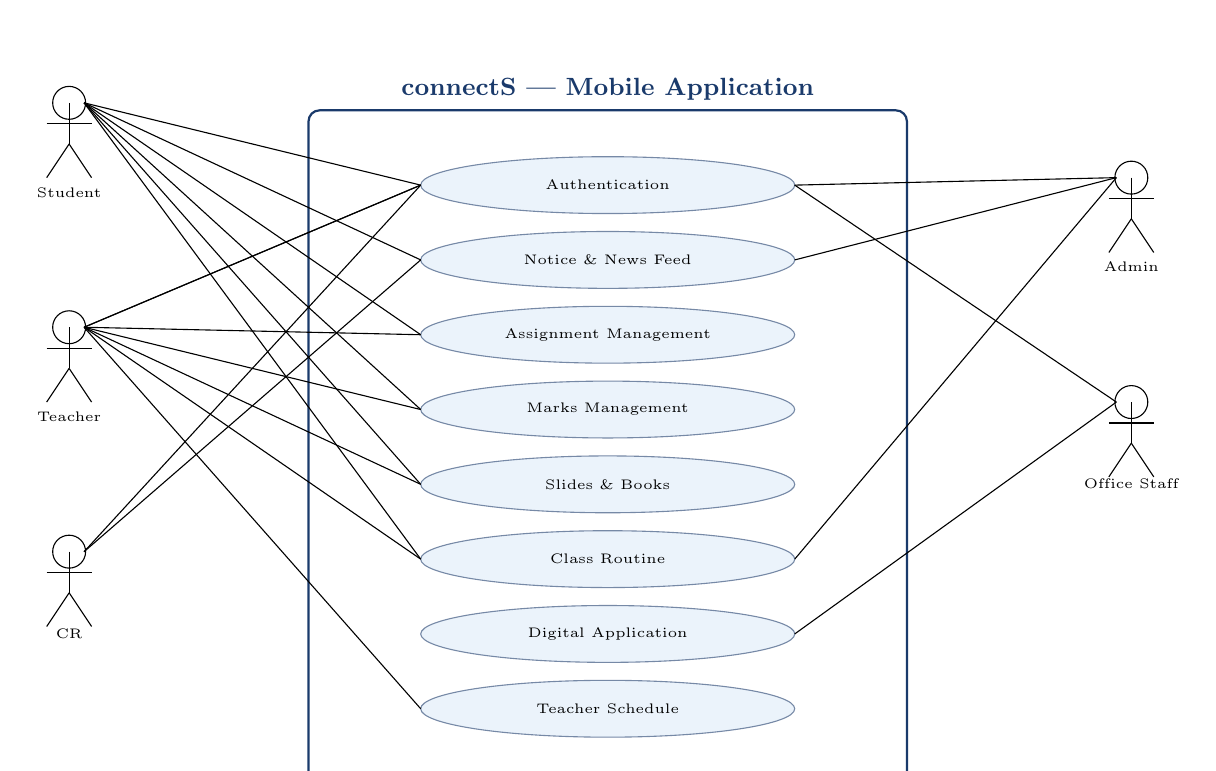
\begin{tikzpicture}[font=\small, scale=0.95]
  \draw[thick, navyblue, rounded corners=4pt] (2,0) rectangle (10,9);
  \node[above, navyblue, font=\small\bfseries] at (6,9) {connectS --- Mobile Application};

  \foreach \y/\name in {8/Authentication, 7/Notice \& News Feed, 6/Assignment Management,
                         5/Marks Management, 4/Slides \& Books, 3/Class Routine,
                         2/Digital Application, 1/Teacher Schedule} {
    \draw[navyblue!60, fill=lightblue] (6,\y) ellipse (2.5cm and 0.38cm);
    \node[font=\tiny] at (6,\y) {\name};
  }

  \node[font=\tiny, below] at (-1.2,8.1) {Student};
  \draw (-1.2,9.1) circle (0.22);
  \draw (-1.2,9.1)--(-1.2,8.55); \draw (-1.2,8.55)--(-1.5,8.1); \draw (-1.2,8.55)--(-0.9,8.1);
  \draw (-1.5,8.82)--(-0.9,8.82);

  \node[font=\tiny, below] at (-1.2,5.1) {Teacher};
  \draw (-1.2,6.1) circle (0.22);
  \draw (-1.2,6.1)--(-1.2,5.55); \draw (-1.2,5.55)--(-1.5,5.1); \draw (-1.2,5.55)--(-0.9,5.1);
  \draw (-1.5,5.82)--(-0.9,5.82);

  \node[font=\tiny, below] at (-1.2,2.2) {CR};
  \draw (-1.2,3.1) circle (0.22);
  \draw (-1.2,3.1)--(-1.2,2.55); \draw (-1.2,2.55)--(-1.5,2.1); \draw (-1.2,2.55)--(-0.9,2.1);
  \draw (-1.5,2.82)--(-0.9,2.82);

  \node[font=\tiny, below] at (13,7.1) {Admin};
  \draw (13,8.1) circle (0.22);
  \draw (13,8.1)--(13,7.55); \draw (13,7.55)--(12.7,7.1); \draw (13,7.55)--(13.3,7.1);
  \draw (12.7,7.82)--(13.3,7.82);

  \node[font=\tiny, below] at (13,4.2) {Office Staff};
  \draw (13,5.1) circle (0.22);
  \draw (13,5.1)--(13,4.55); \draw (13,4.55)--(12.7,4.1); \draw (13,4.55)--(13.3,4.1);
  \draw (12.7,4.82)--(13.3,4.82);

  \foreach \y in {8,7,6,5,4,3} {
    \draw (-1.0,9.1) -- (3.5,\y);
  }
  \foreach \y in {8,6,5,4,3,8} {
    \draw (-1.0,6.1) -- (3.5,\y);
  }
  \draw (-1.0,6.1) -- (3.5,1);
  \draw (-1.0,3.1) -- (3.5,8);
  \draw (-1.0,3.1) -- (3.5,7);
  \draw (12.8,8.1) -- (8.5,8);
  \draw (12.8,8.1) -- (8.5,7);
  \draw (12.8,8.1) -- (8.5,3);
  \draw (12.8,5.1) -- (8.5,8);
  \draw (12.8,5.1) -- (8.5,2);
\end{tikzpicture}
\end{center}

\subsubsection{Level 1 --- User Login and Authentication}

\vspace{0.5em}
\begin{center}
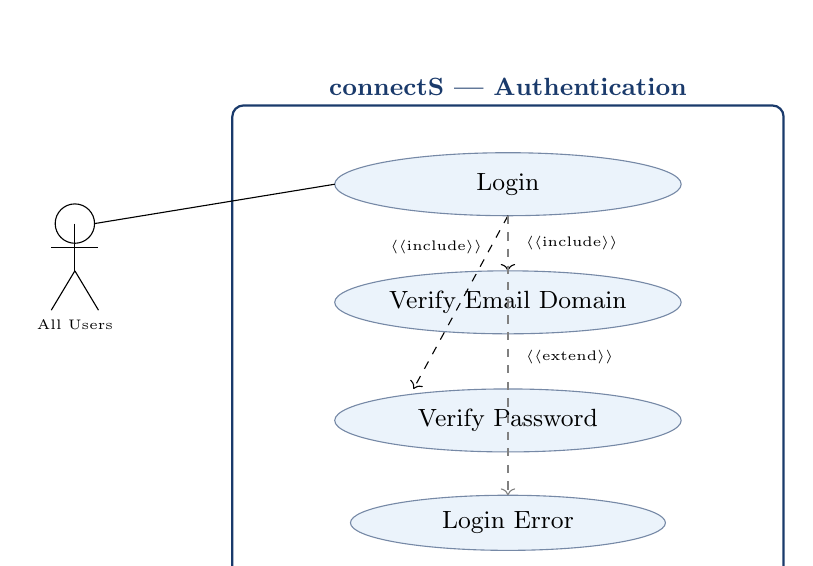
\begin{tikzpicture}[font=\small]
  \draw[thick, navyblue, rounded corners=4pt] (2.5,0) rectangle (9.5,6);
  \node[above, navyblue, font=\small\bfseries] at (6,6) {connectS --- Authentication};

  \draw[navyblue!60, fill=lightblue] (6,5) ellipse (2.2cm and 0.4cm);
  \node[font=\small] at (6,5) {Login};

  \draw[navyblue!60, fill=lightblue] (6,3.5) ellipse (2.2cm and 0.4cm);
  \node[font=\small] at (6,3.5) {Verify Email Domain};

  \draw[navyblue!60, fill=lightblue] (6,2) ellipse (2.2cm and 0.4cm);
  \node[font=\small] at (6,2) {Verify Password};

  \draw[navyblue!60, fill=lightblue] (6,0.7) ellipse (2cm and 0.35cm);
  \node[font=\small] at (6,0.7) {Login Error};

  \draw[->, dashed] (6,4.6) -- (6,3.9);
  \node[right, font=\tiny] at (6.1,4.25) {$\langle\langle$include$\rangle\rangle$};

  \draw[->, dashed] (6,4.6) -- (4.8,2.4);
  \node[left, font=\tiny] at (5.8,4.2) {$\langle\langle$include$\rangle\rangle$};

  \draw[->, dashed, gray] (6,4.6) -- (6,1.05);
  \node[right, font=\tiny] at (6.1,2.8) {$\langle\langle$extend$\rangle\rangle$};

  \draw (0.5,4.5) circle (0.25);
  \draw (0.5,4.5)--(0.5,3.9); \draw (0.5,3.9)--(0.2,3.4); \draw (0.5,3.9)--(0.8,3.4);
  \draw (0.2,4.2)--(0.8,4.2);
  \node[below, font=\tiny] at (0.5,3.4) {All Users};
  \draw (0.75,4.5) -- (3.8,5);
\end{tikzpicture}
\end{center}

\subsubsection{Level 2 --- Assignment Deadline Management}

\vspace{0.5em}
\begin{center}
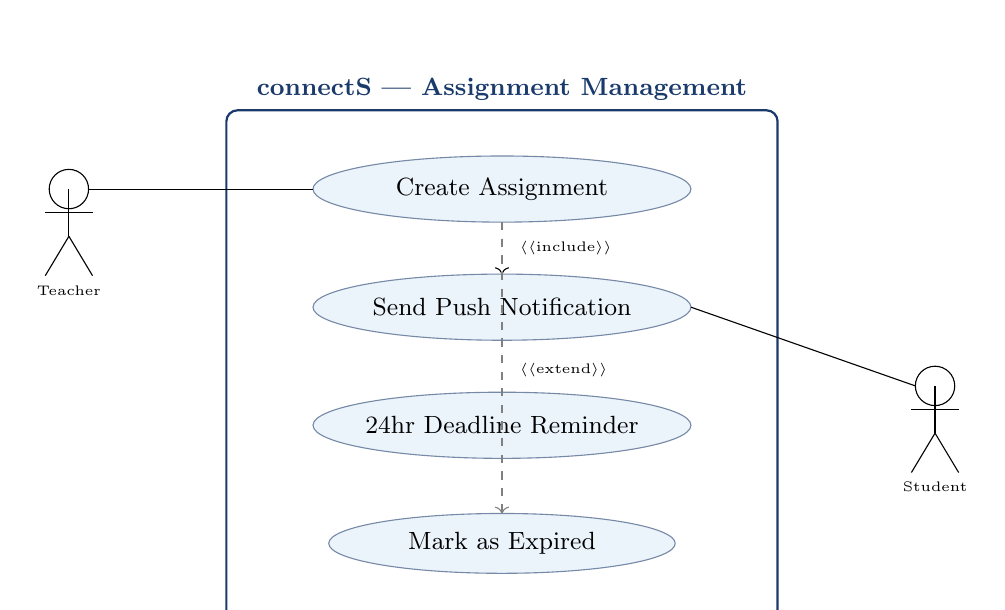
\begin{tikzpicture}[font=\small]
  \draw[thick, navyblue, rounded corners=4pt] (2.5,0) rectangle (9.5,6.5);
  \node[above, navyblue, font=\small\bfseries] at (6,6.5) {connectS --- Assignment Management};

  \draw[navyblue!60, fill=lightblue] (6,5.5) ellipse (2.4cm and 0.42cm);
  \node[font=\small] at (6,5.5) {Create Assignment};

  \draw[navyblue!60, fill=lightblue] (6,4) ellipse (2.4cm and 0.42cm);
  \node[font=\small] at (6,4) {Send Push Notification};

  \draw[navyblue!60, fill=lightblue] (6,2.5) ellipse (2.4cm and 0.42cm);
  \node[font=\small] at (6,2.5) {24hr Deadline Reminder};

  \draw[navyblue!60, fill=lightblue] (6,1) ellipse (2.2cm and 0.38cm);
  \node[font=\small] at (6,1) {Mark as Expired};

  \draw[->, dashed] (6,5.08) -- (6,4.42);
  \node[right, font=\tiny] at (6.1,4.75) {$\langle\langle$include$\rangle\rangle$};

  \draw[->, dashed, gray] (6,5.08) -- (6,1.38);
  \node[right, font=\tiny] at (6.1,3.2) {$\langle\langle$extend$\rangle\rangle$};

  \draw (0.5,5.5) circle (0.25);
  \draw (0.5,5.5)--(0.5,4.9); \draw (0.5,4.9)--(0.2,4.4); \draw (0.5,4.9)--(0.8,4.4);
  \draw (0.2,5.2)--(0.8,5.2);
  \node[below, font=\tiny] at (0.5,4.4) {Teacher};
  \draw (0.75,5.5) -- (3.6,5.5);

  \draw (11.5,3) circle (0.25);
  \draw (11.5,3)--(11.5,2.4); \draw (11.5,2.4)--(11.2,1.9); \draw (11.5,2.4)--(11.8,1.9);
  \draw (11.2,2.7)--(11.8,2.7);
  \node[below, font=\tiny] at (11.5,1.9) {Student};
  \draw (11.25,3) -- (8.4,4);
\end{tikzpicture}
\end{center}

\subsubsection{Level 3 --- Marks Management}

\vspace{0.5em}
\begin{center}
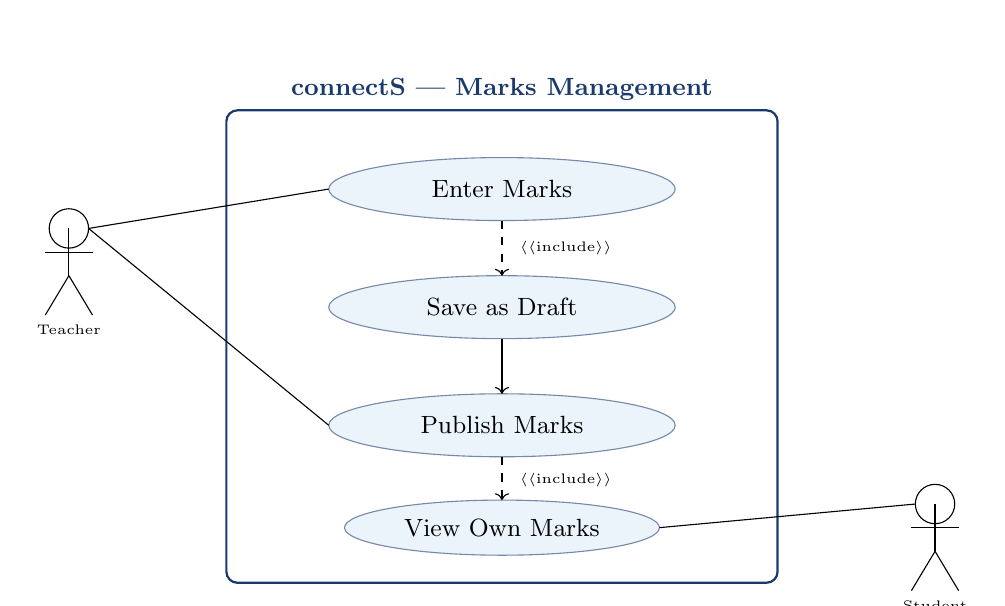
\begin{tikzpicture}[font=\small]
  \draw[thick, navyblue, rounded corners=4pt] (2.5,0) rectangle (9.5,6);
  \node[above, navyblue, font=\small\bfseries] at (6,6) {connectS --- Marks Management};

  \draw[navyblue!60, fill=lightblue] (6,5) ellipse (2.2cm and 0.4cm);
  \node[font=\small] at (6,5) {Enter Marks};

  \draw[navyblue!60, fill=lightblue] (6,3.5) ellipse (2.2cm and 0.4cm);
  \node[font=\small] at (6,3.5) {Save as Draft};

  \draw[navyblue!60, fill=lightblue] (6,2) ellipse (2.2cm and 0.4cm);
  \node[font=\small] at (6,2) {Publish Marks};

  \draw[navyblue!60, fill=lightblue] (6,0.7) ellipse (2cm and 0.35cm);
  \node[font=\small] at (6,0.7) {View Own Marks};

  \draw[->, dashed] (6,4.6) -- (6,3.9);
  \node[right, font=\tiny] at (6.1,4.25) {$\langle\langle$include$\rangle\rangle$};
  \draw[->] (6,3.1) -- (6,2.4);
  \draw[->, dashed] (6,1.6) -- (6,1.05);
  \node[right, font=\tiny] at (6.1,1.3) {$\langle\langle$include$\rangle\rangle$};

  \draw (0.5,4.5) circle (0.25);
  \draw (0.5,4.5)--(0.5,3.9); \draw (0.5,3.9)--(0.2,3.4); \draw (0.5,3.9)--(0.8,3.4);
  \draw (0.2,4.2)--(0.8,4.2);
  \node[below, font=\tiny] at (0.5,3.4) {Teacher};
  \draw (0.75,4.5) -- (3.8,5);
  \draw (0.75,4.5) -- (3.8,2);

  \draw (11.5,1) circle (0.25);
  \draw (11.5,1)--(11.5,0.4); \draw (11.5,0.4)--(11.2,-0.1); \draw (11.5,0.4)--(11.8,-0.1);
  \draw (11.2,0.7)--(11.8,0.7);
  \node[below, font=\tiny] at (11.5,-0.1) {Student};
  \draw (11.25,1) -- (8.0,0.7);
\end{tikzpicture}
\end{center}

\subsubsection{Level 4 --- Digital Application and Approval}

\vspace{0.5em}
\begin{center}
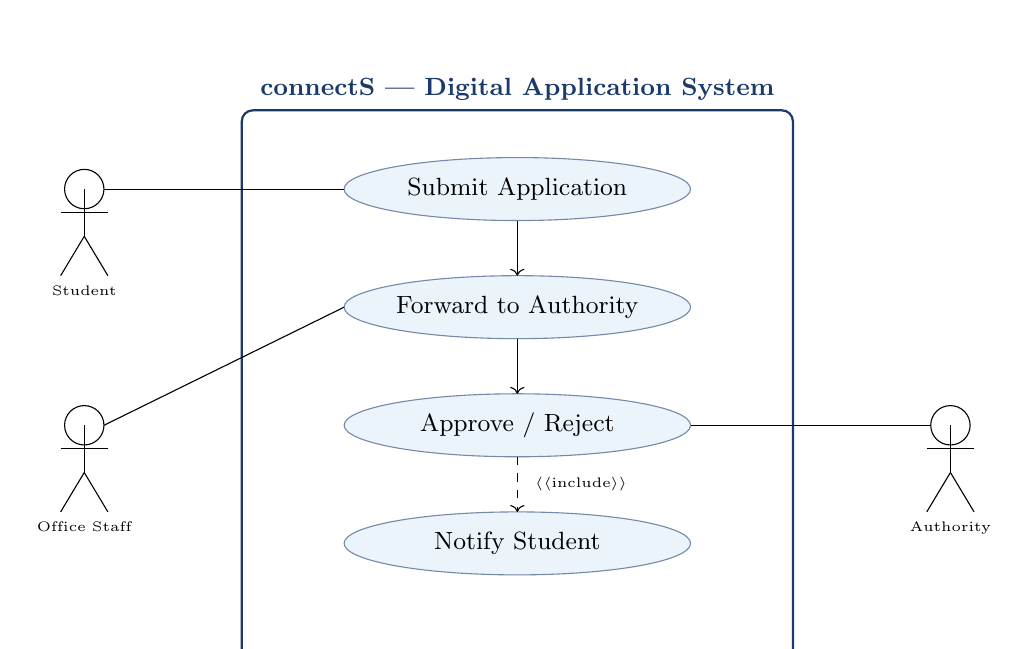
\begin{tikzpicture}[font=\small]
  \draw[thick, navyblue, rounded corners=4pt] (2.5,0) rectangle (9.5,7);
  \node[above, navyblue, font=\small\bfseries] at (6,7) {connectS --- Digital Application System};

  \draw[navyblue!60, fill=lightblue] (6,6) ellipse (2.2cm and 0.4cm);
  \node[font=\small] at (6,6) {Submit Application};

  \draw[navyblue!60, fill=lightblue] (6,4.5) ellipse (2.2cm and 0.4cm);
  \node[font=\small] at (6,4.5) {Forward to Authority};

  \draw[navyblue!60, fill=lightblue] (6,3) ellipse (2.2cm and 0.4cm);
  \node[font=\small] at (6,3) {Approve / Reject};

  \draw[navyblue!60, fill=lightblue] (6,1.5) ellipse (2.2cm and 0.4cm);
  \node[font=\small] at (6,1.5) {Notify Student};

  \draw[->] (6,5.6) -- (6,4.9);
  \draw[->] (6,4.1) -- (6,3.4);
  \draw[->, dashed] (6,2.6) -- (6,1.9);
  \node[right, font=\tiny] at (6.1,2.25) {$\langle\langle$include$\rangle\rangle$};

  \draw (0.5,6) circle (0.25);
  \draw (0.5,6)--(0.5,5.4); \draw (0.5,5.4)--(0.2,4.9); \draw (0.5,5.4)--(0.8,4.9);
  \draw (0.2,5.7)--(0.8,5.7);
  \node[below, font=\tiny] at (0.5,4.9) {Student};
  \draw (0.75,6) -- (3.8,6);

  \draw (0.5,3) circle (0.25);
  \draw (0.5,3)--(0.5,2.4); \draw (0.5,2.4)--(0.2,1.9); \draw (0.5,2.4)--(0.8,1.9);
  \draw (0.2,2.7)--(0.8,2.7);
  \node[below, font=\tiny] at (0.5,1.9) {Office Staff};
  \draw (0.75,3) -- (3.8,4.5);

  \draw (11.5,3) circle (0.25);
  \draw (11.5,3)--(11.5,2.4); \draw (11.5,2.4)--(11.2,1.9); \draw (11.5,2.4)--(11.8,1.9);
  \draw (11.2,2.7)--(11.8,2.7);
  \node[below, font=\tiny] at (11.5,1.9) {Authority};
  \draw (11.25,3) -- (8.2,3);
\end{tikzpicture}
\end{center}
\newpage

%% ============================================================================
%%  CHAPTER 11 — DATA AND CLASS BASED MODELING
%% ============================================================================
\newpage
\section{Data and Class Based Modeling}

\subsection{Data Based Modeling}

\subsubsection{Identify Data Objects}

\begin{center}
\begin{tabular}{llll}
$\bullet$ User & $\bullet$ Notice & $\bullet$ Assignment & $\bullet$ Mark \\
$\bullet$ Slide & $\bullet$ Book & $\bullet$ ClassRoutine & $\bullet$ Course \\
$\bullet$ Application & $\bullet$ TeacherSchedule & $\bullet$ Quiz & $\bullet$ Notification \\
\end{tabular}
\end{center}

\subsubsection{Final Data Objects}

\vspace{0.4em}
\rowcolors{2}{rowalt}{white}
\begin{longtable}{|>{\centering\arraybackslash}p{0.5cm}|p{3.5cm}|p{9.5cm}|}
\hline
\rowcolor{navyblue}
\THH{\#} & \THH{Data Object} & \THH{Attributes} \\
\hline
\endhead
1 & User &
user\_id, name, email, password\_hash, role, batch, phone, profile\_image, handles, created\_at \\
\hline
2 & Notice &
notice\_id, title, body, posted\_by, target, batch\_id, created\_at \\
\hline
3 & Assignment &
assignment\_id, title, description, course\_id, teacher\_id, deadline, is\_expired, created\_at \\
\hline
4 & Mark &
mark\_id, student\_id, course\_id, teacher\_id, assessment\_type, score, is\_published, published\_at \\
\hline
5 & Slide &
slide\_id, title, course\_id, teacher\_id, file\_url, uploaded\_at \\
\hline
6 & Book &
book\_id, title, author, course\_id, uploaded\_by, file\_url, uploaded\_at \\
\hline
7 & ClassRoutine &
routine\_id, semester, file\_url, uploaded\_by, uploaded\_at, version \\
\hline
8 & Course &
course\_id, code, title, credits, semester, prerequisites, teacher\_id \\
\hline
9 & Application &
application\_id, student\_id, type, description, status, assigned\_to, office\_staff\_id, comment, submitted\_at, resolved\_at \\
\hline
10 & TeacherSchedule &
schedule\_id, teacher\_id, weekly\_slots, next\_day\_availability, updated\_at \\
\hline
11 & Quiz &
quiz\_id, title, course\_id, teacher\_id, questions, created\_at \\
\hline
12 & Notification &
notif\_id, user\_id, title, body, type, is\_read, created\_at \\
\hline
\end{longtable}

\subsection{Class Based Modeling}

\subsubsection{Final Classes}

\vspace{0.4em}
\rowcolors{2}{rowalt}{white}
\begin{longtable}{|p{2.8cm}|p{5.5cm}|p{5.2cm}|}
\hline
\rowcolor{navyblue}
\THH{Class} & \THH{Key Attributes} & \THH{Key Methods} \\
\hline
\endhead
User &
-user\_id: int \newline
-name: string \newline
-email: string \newline
-password\_hash: string \newline
-role: enum \newline
-batch: string &
+login(): bool \newline
+logout(): void \newline
+updateProfile(): void \newline
+updateHandles(): void \newline
+getRole(): string \\
\hline
Notice &
-notice\_id: int \newline
-title: string \newline
-body: string \newline
-posted\_by: int \newline
-target: enum \newline
-batch\_id: string &
+create(): void \newline
+publish(): void \newline
+delete(): void \newline
+getAll(): Notice[] \newline
+getByBatch(): Notice[] \\
\hline
Assignment &
-assignment\_id: int \newline
-title: string \newline
-description: string \newline
-course\_id: int \newline
-deadline: datetime \newline
-is\_expired: bool &
+create(): void \newline
+update(): void \newline
+delete(): void \newline
+getActive(): Assignment[] \newline
+markExpired(): void \\
\hline
Mark &
-mark\_id: int \newline
-student\_id: int \newline
-assessment\_type: string \newline
-score: float \newline
-is\_published: bool &
+enter(): void \newline
+saveDraft(): void \newline
+publish(): void \newline
+getByStudent(): Mark[] \\
\hline
Slide &
-slide\_id: int \newline
-title: string \newline
-course\_id: int \newline
-teacher\_id: int \newline
-file\_url: string &
+upload(): void \newline
+delete(): void \newline
+getByCourse(): Slide[] \newline
+download(): void \\
\hline
Book &
-book\_id: int \newline
-title: string \newline
-author: string \newline
-course\_id: int \newline
-file\_url: string &
+upload(): void \newline
+replace(): void \newline
+delete(): void \newline
+getByCourse(): Book[] \\
\hline
Course &
-course\_id: int \newline
-code: string \newline
-title: string \newline
-credits: int \newline
-semester: int \newline
-teacher\_id: int &
+add(): void \newline
+update(): void \newline
+archive(): void \newline
+search(): Course[] \newline
+filterBySemester(): Course[] \\
\hline
Application &
-application\_id: int \newline
-student\_id: int \newline
-type: string \newline
-status: enum \newline
-assigned\_to: int &
+submit(): void \newline
+forward(): void \newline
+approve(): void \newline
+reject(): void \newline
+getStatus(): string \\
\hline
TeacherSchedule &
-schedule\_id: int \newline
-teacher\_id: int \newline
-weekly\_slots: JSON \newline
-next\_day: JSON &
+update(): void \newline
+updateNextDay(): void \newline
+getByTeacher(): Schedule \\
\hline
Notification &
-notif\_id: int \newline
-user\_id: int \newline
-title: string \newline
-type: string \newline
-is\_read: bool &
+send(): void \newline
+markRead(): void \newline
+getUnread(): Notification[] \\
\hline
Quiz &
-quiz\_id: int \newline
-title: string \newline
-course\_id: int \newline
-questions: JSON &
+create(): void \newline
+publish(): void \newline
+attempt(): void \newline
+getResult(): float \\
\hline
\end{longtable}
\newpage

%% ============================================================================
%%  CHAPTER 12 — ARCHITECTURAL DESIGN
%% ============================================================================
\newpage
\section{Architectural Design}

\subsection{Representing the System in Context}

\vspace{0.5em}
\begin{center}
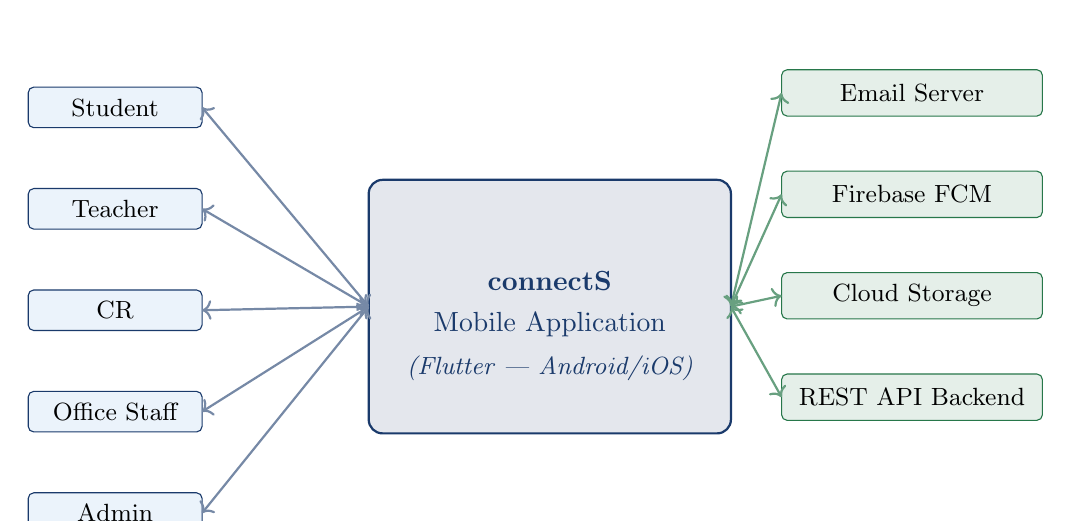
\begin{tikzpicture}[font=\small, scale=0.92]

  \draw[fill=navyblue!12, draw=navyblue, thick, rounded corners=5pt] (3.5,2.5) rectangle (8.5,6);
  \node[navyblue, font=\bfseries] at (6,4.6) {connectS};
  \node[navyblue, font=\normalsize] at (6,4.0) {Mobile Application};
  \node[navyblue, font=\small\itshape] at (6,3.4) {(Flutter --- Android/iOS)};

  \foreach \y/\name in {7.0/Student, 5.6/Teacher, 4.2/CR, 2.8/Office Staff, 1.4/Admin} {
    \draw[fill=lightblue, draw=navyblue, rounded corners=2pt] (-1.2,\y-0.28) rectangle (1.2,\y+0.28);
    \node[font=\small] at (0,\y) {\name};
    \draw[<->, thick, navyblue!60] (1.2,\y) -- (3.5,4.25);
  }

  \foreach \y/\name in {7.2/Email Server, 5.8/Firebase FCM, 4.4/Cloud Storage, 3.0/REST API Backend} {
    \draw[fill=successgreen!12, draw=successgreen, rounded corners=2pt] (9.2,\y-0.32) rectangle (12.8,\y+0.32);
    \node[font=\small] at (11,\y) {\name};
    \draw[<->, thick, successgreen!70] (8.5,4.25) -- (9.2,\y);
  }

\end{tikzpicture}
\end{center}

\subsection{Mapping Requirements to Software Architecture}

\vspace{0.4em}
\rowcolors{2}{rowalt}{white}
\begin{longtable}{|p{4.5cm}|p{3.8cm}|p{5.2cm}|}
\hline
\rowcolor{navyblue}
\THH{Functional Requirement} & \THH{Component} & \THH{Technology / Approach} \\
\hline
\endhead
Institutional email login and role assignment &
Auth Module &
Email domain check, JWT session token, bcrypt password hashing \\
\hline
Push notifications for deadlines and notices &
Notification Module &
Firebase Cloud Messaging (FCM), background scheduler \\
\hline
Official notice board and CR news feed &
Notice Module &
REST API, role and batch-based access filter \\
\hline
Assignment creation and deadline tracking &
Assignment Module &
REST API, scheduled background job for reminders \\
\hline
Marks entry and publication &
Marks Module &
REST API, draft/publish state machine, student-ID filter \\
\hline
Lecture slide upload and in-app viewing &
Slide Module &
Cloud Storage, in-app PDF viewer \\
\hline
Books PDF library by course &
Resource Module &
Cloud Storage, lazy-loading PDF viewer \\
\hline
Class routine upload and update &
Routine Module &
Cloud Storage, Admin-only upload API, FCM on update \\
\hline
Course catalogue with search and filter &
Course Module &
REST API, client-side keyword search and semester filter \\
\hline
Teacher schedule and consultation hours &
Schedule Module &
REST API, real-time polling for live updates \\
\hline
Digital application and approval workflow &
Application Module &
REST API, multi-step status machine, FCM at each stage \\
\hline
Student professional handles &
Profile Module &
REST API, dynamic URL builder, external browser link \\
\hline
Dark mode and light mode &
Theme Module &
Flutter ThemeData, SharedPreferences for persistence \\
\hline
Mini quiz feature &
Quiz Module &
REST API, JSON question storage, auto-score calculation \\
\hline
\end{longtable}
\newpage

%% ============================================================================
%%  CHAPTER 13 — TESTING PLAN
%% ============================================================================
\newpage
\section{Testing Plan}

\subsection{High-Level Description of Testing Goals}

\begin{itemize}[leftmargin=*, label=\textbullet, itemsep=4pt]
  \item \textbf{Bug Prevention:} Test each feature as soon as it is built to catch errors before they affect other parts of the system.
  \item \textbf{User Satisfaction:} Verify that the system behaves exactly as stakeholders described during elicitation interviews.
  \item \textbf{Security:} Confirm that role-based access control works correctly and no user can access another user's data.
  \item \textbf{Performance:} Verify that the app loads the main screen in under 3 seconds on a slow 3G network.
  \item \textbf{Reliability:} Test that the system stays available during peak usage hours and handles network errors gracefully.
\end{itemize}

\subsection{Sample Test Cases}

\vspace{0.4em}
\rowcolors{2}{rowalt}{white}
\begin{longtable}{|>{\centering\arraybackslash}p{1cm}|p{2.8cm}|p{3cm}|p{2.5cm}|p{2.5cm}|>{\centering\arraybackslash}p{1cm}|}
\hline
\rowcolor{navyblue}
\THH{TC ID} & \THH{Scenario} & \THH{Steps} & \THH{Expected Output} & \THH{Actual Output} & \THH{Result} \\
\hline
\endhead
TC-01 &
Login with valid institutional email &
Enter valid email and correct password, tap Login &
User reaches role-specific home screen &
Same as expected &
Pass \\
\hline
TC-02 &
Login with invalid email domain &
Enter an email from a different domain, tap Login &
Error: "Only allowed email domains are accepted" &
Same as expected &
Pass \\
\hline
TC-03 &
Student tries to access another student's marks &
Log in as Student A, try to fetch Student B's marks via API &
Access denied; only own marks returned &
Same as expected &
Pass \\
\hline
TC-04 &
Teacher publishes marks &
Enter marks, save as draft, tap Publish &
Marks visible to students; push notification sent &
Same as expected &
Pass \\
\hline
TC-05 &
CR posts batch notice &
Log in as CR, write notice, post &
Notice visible only to own batch &
Same as expected &
Pass \\
\hline
TC-06 &
Student submits application &
Fill application form, tap Submit &
Administrative dashboard shows new entry &
Same as expected &
Pass \\
\hline
TC-07 &
Authority approves application &
Open assigned application, tap Approve &
Status changes to Approved; student receives notification &
Same as expected &
Pass \\
\hline
TC-08 &
Dark mode toggle and persistence &
Open settings, enable dark mode, close and reopen app &
Dark mode applied on reopen &
Same as expected &
Pass \\
\hline
\end{longtable}
\newpage

%% ============================================================================
%%  CONCLUSION
%% ============================================================================
\newpage
\section*{Conclusion}
\addcontentsline{toc}{section}{Conclusion}

Preparing this Software Requirements Specification has been a challenging and rewarding experience. The report covers the complete requirements and design modeling of \textbf{connectS}, a Flutter-based mobile application that addresses real and verified problems faced by academic institutions and departments.

Through stakeholder interviews with students, teachers, administrators, and staff, combined with surveys, the team gathered and confirmed 12 in-scope features, 31 functional requirements, and 14 non-functional requirements. The use case diagrams, data object models, class-based models, and architectural design presented in this report provide a clear and structured foundation for the development phase.

The unique findings from elicitation --- such as the digital application and approval system identified from administrative staff interviews, and the dark/light mode requested independently by all stakeholder groups --- show that the requirements gathering process was thorough and effective.

connectS is not only an academic exercise. It is a direct response to problems that students, teachers, and administrators face every day. With careful implementation following this specification, the application will significantly improve academic communication, resource access, and administrative efficiency for academic institutions.

%% ============================================================================
%%  REFERENCES
%% ============================================================================
\newpage
\section*{References}
\addcontentsline{toc}{section}{References}

\begin{enumerate}[leftmargin=*, label={[\arabic*]}, itemsep=5pt]
  \item Pressman, R. S., \& Maxim, B. R. (2015). \textit{Software Engineering: A Practitioner's Approach} (8th ed.). McGraw-Hill Education.
  \item IEEE. (1998). \textit{IEEE Recommended Practice for Software Requirements Specifications} (IEEE Std 830-1998). IEEE Computer Society.
  \item Sommerville, I. (2016). \textit{Software Engineering} (10th ed.). Pearson Education Limited.
  \item Flutter Development Team. (2026). \textit{Flutter Documentation}. Retrieved from \url{https://flutter.dev/docs}
  \item Firebase. (2026). \textit{Firebase Cloud Messaging Documentation}. Retrieved from \url{https://firebase.google.com/docs/cloud-messaging}
  \item Wiegers, K., \& Beatty, J. (2013). \textit{Software Requirements} (3rd ed.). Microsoft Press.
\end{enumerate}

%% ============================================================================
%%  APPENDIX A: GLOSSARY
%% ============================================================================
\newpage
\section*{Appendix A: Glossary}
\addcontentsline{toc}{section}{Appendix A: Glossary}

\begin{longtable}{|p{3.5cm}|p{10.5cm}|}
\hline
\rowcolor{navyblue}
\THH{Term} & \THH{Definition} \\
\hline
\endhead
Admin & User role responsible for system administration, user management, content moderation, and system configuration. \\
\hline
API & Application Programming Interface; defines how software components interact and exchange data. \\
\hline
Assessment & Evaluation of student performance (e.g., Class Test, Continuous Assessment, quizzes). \\
\hline
Batch & A group of students enrolled in the same academic program, year, and section. \\
\hline
bcrypt & A cryptographic hashing function used for securely storing passwords. \\
\hline
CA & Continuous Assessment; ongoing evaluation of student performance throughout the semester. \\
\hline
CR & Class Representative; a student elected to represent their batch and act as a liaison between students and faculty. \\
\hline
CT & Class Test; periodic tests administered during the semester to assess student learning. \\
\hline
Data Dictionary & A centralized repository of information about data elements and their relationships. \\
\hline
FCM & Firebase Cloud Messaging; a cross-platform messaging solution for delivering push notifications. \\
\hline
Flutter & An open-source UI software development toolkit by Google for building cross-platform applications. \\
\hline
FR & Functional Requirement; a specific behavior or function the system must provide. \\
\hline
HTTPS & Hypertext Transfer Protocol Secure; an extension of HTTP for secure communication over a network. \\
\hline
JSON & JavaScript Object Notation; a lightweight data interchange format. \\
\hline
JWT & JSON Web Token; an open standard for securely transmitting information between parties as a JSON object. \\
\hline
Lazy Loading & A design pattern where content is loaded only when needed to improve performance. \\
\hline
Localization & The process of adapting software for a specific region or language. \\
\hline
Material Design & A design language developed by Google for creating consistent user interfaces. \\
\hline
MoSCoW & A prioritization method: Must have, Should have, Could have, Won't have. \\
\hline
NFR & Non-Functional Requirement; defines quality attributes and constraints of the system. \\
\hline
PDF & Portable Document Format; a file format used for presenting documents. \\
\hline
PUC & Product Use Case; describes a specific interaction between a user and the system. \\
\hline
QFD & Quality Function Deployment; a method for translating customer needs into technical requirements. \\
\hline
REST & Representational State Transfer; an architectural style for designing networked applications. \\
\hline
Role & A user classification that determines access permissions and available features. \\
\hline
SRS & Software Requirements Specification; this document. \\
\hline
TLS & Transport Layer Security; a cryptographic protocol for secure communication over a network. \\
\hline
UFTB & University of Frontier Technology, Bangladesh. \\
\hline
Unicode & A standard for consistent encoding, representation, and handling of text in most writing systems. \\
\hline
\end{longtable}

%% ============================================================================
%%  APPENDIX B: ANALYSIS MODELS
%% ============================================================================
\newpage
\section*{Appendix B: Analysis Models}
\addcontentsline{toc}{section}{Appendix B: Analysis Models}

This appendix contains analysis models that support the requirements specification.

\subsection{System Architecture in Context}

\begin{center}
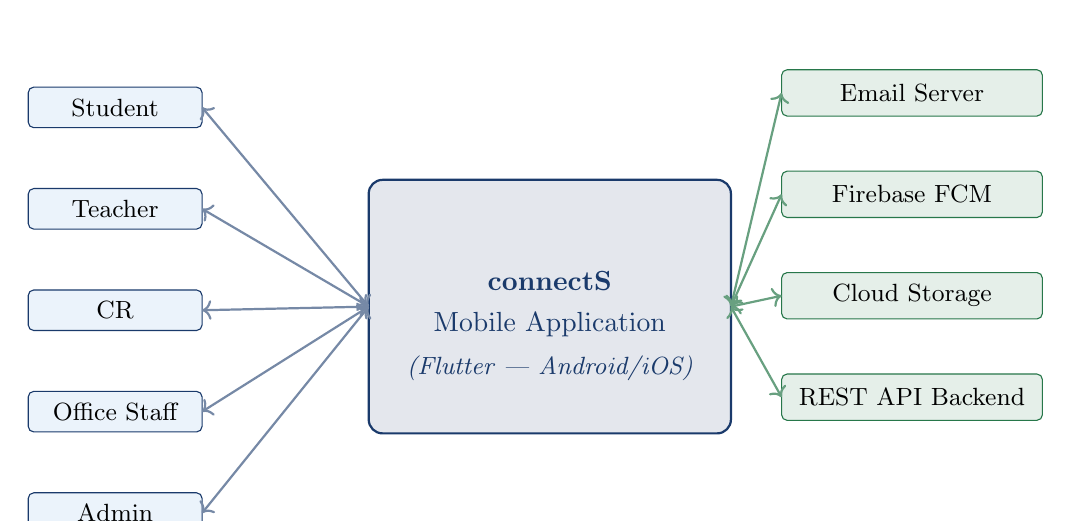
\begin{tikzpicture}[font=\small, scale=0.92]

  \draw[fill=navyblue!12, draw=navyblue, thick, rounded corners=5pt] (3.5,2.5) rectangle (8.5,6);
  \node[navyblue, font=\bfseries] at (6,4.6) {connectS};
  \node[navyblue, font=\normalsize] at (6,4.0) {Mobile Application};
  \node[navyblue, font=\small\itshape] at (6,3.4) {(Flutter --- Android/iOS)};

  \foreach \y/\name in {7.0/Student, 5.6/Teacher, 4.2/CR, 2.8/Office Staff, 1.4/Admin} {
    \draw[fill=lightblue, draw=navyblue, rounded corners=2pt] (-1.2,\y-0.28) rectangle (1.2,\y+0.28);
    \node[font=\small] at (0,\y) {\name};
    \draw[<->, thick, navyblue!60] (1.2,\y) -- (3.5,4.25);
  }

  \foreach \y/\name in {7.2/Email Server, 5.8/Firebase FCM, 4.4/Cloud Storage, 3.0/REST API Backend} {
    \draw[fill=successgreen!12, draw=successgreen, rounded corners=2pt] (9.2,\y-0.32) rectangle (12.8,\y+0.32);
    \node[font=\small] at (11,\y) {\name};
    \draw[<->, thick, successgreen!70] (8.5,4.25) -- (9.2,\y);
  }

\end{tikzpicture}
\end{center}

\subsection{Component Architecture}

\begin{center}
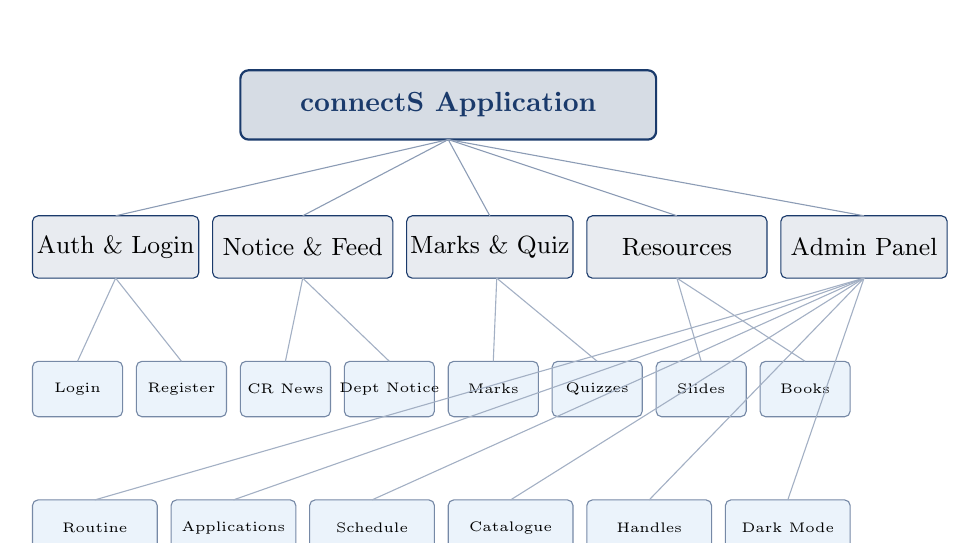
\begin{tikzpicture}[font=\small, scale=0.88]

  \draw[fill=navyblue!18, draw=navyblue, thick, rounded corners=3pt] (3,9) rectangle (9,10);
  \node[font=\bfseries\normalsize, navyblue] at (6,9.5) {connectS Application};

  \foreach \x/\w/\name in {0/2.4/Auth \& Login, 2.6/2.6/Notice \& Feed,
                             5.4/2.4/Marks \& Quiz, 8.0/2.6/Resources,
                             10.8/2.4/Admin Panel} {
    \draw[fill=navyblue!10, draw=navyblue, rounded corners=2pt] (\x,7) rectangle (\x+\w,7.9);
    \node[font=\small] at (\x+\w/2, 7.45) {\name};
    \draw[navyblue!50] (6,9) -- (\x+\w/2,7.9);
  }

  \foreach \x/\name in {0/Login, 1.5/Register, 3/CR News, 4.5/Dept Notice,
                         6/Marks, 7.5/Quizzes, 9/Slides, 10.5/Books} {
    \draw[fill=lightblue, draw=navyblue!60, rounded corners=2pt] (\x,5) rectangle (\x+1.3,5.8);
    \node[font=\tiny] at (\x+0.65,5.4) {\name};
  }
  \draw[navyblue!40] (1.2,7) -- (0.65,5.8);
  \draw[navyblue!40] (1.2,7) -- (2.15,5.8);
  \draw[navyblue!40] (3.9,7) -- (3.65,5.8);
  \draw[navyblue!40] (3.9,7) -- (5.15,5.8);
  \draw[navyblue!40] (6.7,7) -- (6.65,5.8);
  \draw[navyblue!40] (6.7,7) -- (8.15,5.8);
  \draw[navyblue!40] (9.3,7) -- (9.65,5.8);
  \draw[navyblue!40] (9.3,7) -- (11.15,5.8);

  \foreach \x/\name in {0/Routine, 2/Applications, 4/Schedule,
                         6/Catalogue, 8/Handles, 10/Dark Mode} {
    \draw[fill=lightblue, draw=navyblue!60, rounded corners=2pt] (\x,3) rectangle (\x+1.8,3.8);
    \node[font=\tiny] at (\x+0.9,3.4) {\name};
    \draw[navyblue!40] (11.4+1.2/2,7) -- (\x+0.9,3.8);
  }

\end{tikzpicture}
\end{center}

\subsection{Entity-Relationship Diagram}

\begin{center}
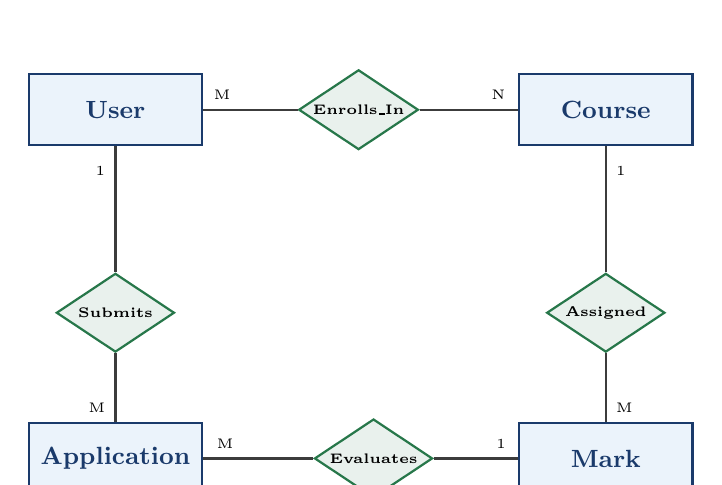
\begin{tikzpicture}[
  node distance=2.2cm and 2.0cm,
  entity/.style={rectangle, draw=navyblue, fill=lightblue, thick, minimum width=2.2cm, minimum height=0.9cm, font=\small\bfseries\color{navyblue}},
  relationship/.style={diamond, draw=successgreen, fill=successgreen!10, thick, minimum width=1.5cm, minimum height=1cm, aspect=1.5, font=\tiny\bfseries, inner sep=1pt},
  line/.style={draw=darkgray, thick}
]

  \node[entity] (user) {User};
  \node[entity, right=4.0cm of user] (course) {Course};
  \node[entity, below=3.5cm of user] (app) {Application};
  \node[entity, below=3.5cm of course] (mark) {Mark};

  \node[relationship, right=1.2cm of user] (enrolled) {Enrolls\_In};
  \node[relationship, below=1.6cm of user] (submits) {Submits};
  \node[relationship, below=1.6cm of course] (has) {Assigned};
  \node[relationship, right=1.4cm of app] (reviews) {Evaluates};

  \path[line] (user) -- (enrolled) node[above, pos=0.2, font=\tiny] {M};
  \path[line] (enrolled) -- (course) node[above, pos=0.8, font=\tiny] {N};
  \path[line] (user) -- (submits) node[left, pos=0.2, font=\tiny] {1};
  \path[line] (submits) -- (app) node[left, pos=0.8, font=\tiny] {M};
  \path[line] (course) -- (has) node[right, pos=0.2, font=\tiny] {1};
  \path[line] (has) -- (mark) node[right, pos=0.8, font=\tiny] {M};
  \path[line] (app) -- (reviews) node[above, pos=0.2, font=\tiny] {M};
  \path[line] (reviews) -- (mark) node[above, pos=0.8, font=\tiny] {1};

\end{tikzpicture}
\end{center}

\subsection{Use Case Diagram --- System Overview}

\begin{center}
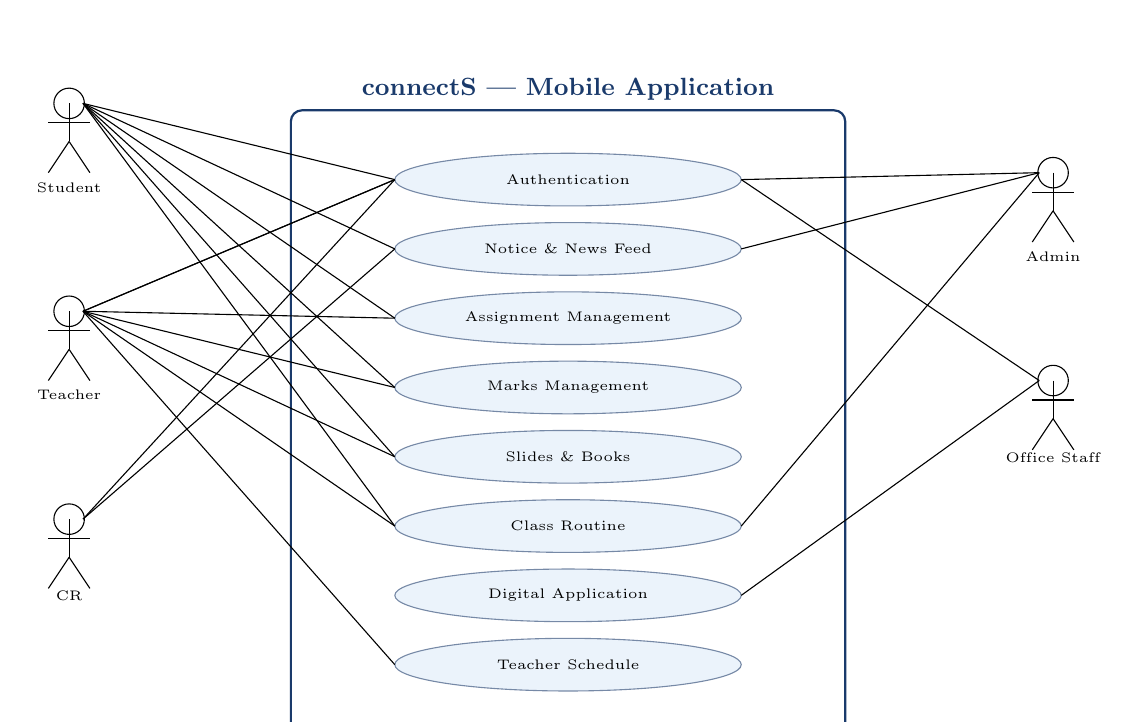
\begin{tikzpicture}[font=\small, scale=0.88]
  \draw[thick, navyblue, rounded corners=4pt] (2,0) rectangle (10,9);
  \node[above, navyblue, font=\small\bfseries] at (6,9) {connectS --- Mobile Application};

  \foreach \y/\name in {8/Authentication, 7/Notice \& News Feed, 6/Assignment Management,
                         5/Marks Management, 4/Slides \& Books, 3/Class Routine,
                         2/Digital Application, 1/Teacher Schedule} {
    \draw[navyblue!60, fill=lightblue] (6,\y) ellipse (2.5cm and 0.38cm);
    \node[font=\tiny] at (6,\y) {\name};
  }

  \node[font=\tiny, below] at (-1.2,8.1) {Student};
  \draw (-1.2,9.1) circle (0.22);
  \draw (-1.2,9.1)--(-1.2,8.55); \draw (-1.2,8.55)--(-1.5,8.1); \draw (-1.2,8.55)--(-0.9,8.1);
  \draw (-1.5,8.82)--(-0.9,8.82);

  \node[font=\tiny, below] at (-1.2,5.1) {Teacher};
  \draw (-1.2,6.1) circle (0.22);
  \draw (-1.2,6.1)--(-1.2,5.55); \draw (-1.2,5.55)--(-1.5,5.1); \draw (-1.2,5.55)--(-0.9,5.1);
  \draw (-1.5,5.82)--(-0.9,5.82);

  \node[font=\tiny, below] at (-1.2,2.2) {CR};
  \draw (-1.2,3.1) circle (0.22);
  \draw (-1.2,3.1)--(-1.2,2.55); \draw (-1.2,2.55)--(-1.5,2.1); \draw (-1.2,2.55)--(-0.9,2.1);
  \draw (-1.5,2.82)--(-0.9,2.82);

  \node[font=\tiny, below] at (13,7.1) {Admin};
  \draw (13,8.1) circle (0.22);
  \draw (13,8.1)--(13,7.55); \draw (13,7.55)--(12.7,7.1); \draw (13,7.55)--(13.3,7.1);
  \draw (12.7,7.82)--(13.3,7.82);

  \node[font=\tiny, below] at (13,4.2) {Office Staff};
  \draw (13,5.1) circle (0.22);
  \draw (13,5.1)--(13,4.55); \draw (13,4.55)--(12.7,4.1); \draw (13,4.55)--(13.3,4.1);
  \draw (12.7,4.82)--(13.3,4.82);

  \foreach \y in {8,7,6,5,4,3} {
    \draw (-1.0,9.1) -- (3.5,\y);
  }
  \foreach \y in {8,6,5,4,3,8} {
    \draw (-1.0,6.1) -- (3.5,\y);
  }
  \draw (-1.0,6.1) -- (3.5,1);
  \draw (-1.0,3.1) -- (3.5,8);
  \draw (-1.0,3.1) -- (3.5,7);
  \draw (12.8,8.1) -- (8.5,8);
  \draw (12.8,8.1) -- (8.5,7);
  \draw (12.8,8.1) -- (8.5,3);
  \draw (12.8,5.1) -- (8.5,8);
  \draw (12.8,5.1) -- (8.5,2);
\end{tikzpicture}
\end{center}

%% ============================================================================
%%  END OF DOCUMENT
%% ============================================================================
\end{document}